\documentclass[twoside]{book}

% Packages required by doxygen
\usepackage{calc}
\usepackage{doxygen}
\usepackage{graphicx}
\usepackage[utf8]{inputenc}
\usepackage{makeidx}
\usepackage{multicol}
\usepackage{multirow}
\usepackage{textcomp}
\usepackage[table]{xcolor}

% Font selection
\usepackage[T1]{fontenc}
\usepackage{mathptmx}
\usepackage[scaled=.90]{helvet}
\usepackage{courier}
\usepackage{amssymb}
\usepackage{sectsty}
\renewcommand{\familydefault}{\sfdefault}
\allsectionsfont{%
  \fontseries{bc}\selectfont%
  \color{darkgray}%
}
\renewcommand{\DoxyLabelFont}{%
  \fontseries{bc}\selectfont%
  \color{darkgray}%
}

% Page & text layout
\usepackage{geometry}
\geometry{%
  a4paper,%
  top=2.5cm,%
  bottom=2.5cm,%
  left=2.5cm,%
  right=2.5cm%
}
\tolerance=750
\hfuzz=15pt
\hbadness=750
\setlength{\emergencystretch}{15pt}
\setlength{\parindent}{0cm}
\setlength{\parskip}{0.2cm}
\makeatletter
\renewcommand{\paragraph}{%
  \@startsection{paragraph}{4}{0ex}{-1.0ex}{1.0ex}{%
    \normalfont\normalsize\bfseries\SS@parafont%
  }%
}
\renewcommand{\subparagraph}{%
  \@startsection{subparagraph}{5}{0ex}{-1.0ex}{1.0ex}{%
    \normalfont\normalsize\bfseries\SS@subparafont%
  }%
}
\makeatother

% Headers & footers
\usepackage{fancyhdr}
\pagestyle{fancyplain}
\fancyhead[LE]{\fancyplain{}{\bfseries\thepage}}
\fancyhead[CE]{\fancyplain{}{}}
\fancyhead[RE]{\fancyplain{}{\bfseries\leftmark}}
\fancyhead[LO]{\fancyplain{}{\bfseries\rightmark}}
\fancyhead[CO]{\fancyplain{}{}}
\fancyhead[RO]{\fancyplain{}{\bfseries\thepage}}
\fancyfoot[LE]{\fancyplain{}{}}
\fancyfoot[CE]{\fancyplain{}{}}
\fancyfoot[RE]{\fancyplain{}{\bfseries\scriptsize Generated on Mon Mar 9 2015 23\-:11\-:52 for Robot Simulation by Doxygen }}
\fancyfoot[LO]{\fancyplain{}{\bfseries\scriptsize Generated on Mon Mar 9 2015 23\-:11\-:52 for Robot Simulation by Doxygen }}
\fancyfoot[CO]{\fancyplain{}{}}
\fancyfoot[RO]{\fancyplain{}{}}
\renewcommand{\footrulewidth}{0.4pt}
\renewcommand{\chaptermark}[1]{%
  \markboth{#1}{}%
}
\renewcommand{\sectionmark}[1]{%
  \markright{\thesection\ #1}%
}

% Indices & bibliography
\usepackage{natbib}
\usepackage[titles]{tocloft}
\setcounter{tocdepth}{3}
\setcounter{secnumdepth}{5}
\makeindex

% Hyperlinks (required, but should be loaded last)
\usepackage{ifpdf}
\ifpdf
  \usepackage[pdftex,pagebackref=true]{hyperref}
\else
  \usepackage[ps2pdf,pagebackref=true]{hyperref}
\fi
\hypersetup{%
  colorlinks=true,%
  linkcolor=blue,%
  citecolor=blue,%
  unicode%
}

% Custom commands
\newcommand{\clearemptydoublepage}{%
  \newpage{\pagestyle{empty}\cleardoublepage}%
}


%===== C O N T E N T S =====

\begin{document}

% Titlepage & ToC
\hypersetup{pageanchor=false}
\pagenumbering{roman}
\begin{titlepage}
\vspace*{7cm}
\begin{center}%
{\Large Robot Simulation }\\
\vspace*{1cm}
{\large Generated by Doxygen 1.8.6}\\
\vspace*{0.5cm}
{\small Mon Mar 9 2015 23:11:52}\\
\end{center}
\end{titlepage}
\clearemptydoublepage
\tableofcontents
\clearemptydoublepage
\pagenumbering{arabic}
\hypersetup{pageanchor=true}

%--- Begin generated contents ---
\chapter{\char`\"{}\-Robot Simulation Documentation File\char`\"{}}
\label{index}\hypertarget{index}{}\subsection*{Authors}

Nicole Zhang Rachel Soble Nicholas Inman

\subsection*{This is the documentation file for our robot simulator.}

Here you will find documentation on Group 5's robot simulator.


\chapter{R\-E\-A\-D\-M\-E}
\label{md_README}
\hypertarget{md_README}{}
sdfk;jasfdkj;lsajflskdjfl\-:q 
\chapter{Hierarchical Index}
\section{Class Hierarchy}
This inheritance list is sorted roughly, but not completely, alphabetically\-:\begin{DoxyCompactList}
\item \contentsline{section}{Base\-Gfx\-App}{\pageref{classBaseGfxApp}}{}
\begin{DoxyCompactList}
\item \contentsline{section}{Simulation}{\pageref{classSimulation}}{}
\end{DoxyCompactList}
\item \contentsline{section}{Environment\-Class}{\pageref{classEnvironmentClass}}{}
\item \contentsline{section}{Physical\-Object\-Class}{\pageref{classPhysicalObjectClass}}{}
\begin{DoxyCompactList}
\item \contentsline{section}{Obstacle\-Class}{\pageref{classObstacleClass}}{}
\item \contentsline{section}{Robot\-Class}{\pageref{classRobotClass}}{}
\item \contentsline{section}{Target\-Class}{\pageref{classTargetClass}}{}
\end{DoxyCompactList}
\item \contentsline{section}{Rendering\-Window\-Class}{\pageref{classRenderingWindowClass}}{}
\item Test\-Suite\begin{DoxyCompactList}
\item \contentsline{section}{Obstacle\-Class\-Tests}{\pageref{classObstacleClassTests}}{}
\end{DoxyCompactList}
\item Test\-Suite\begin{DoxyCompactList}
\item \contentsline{section}{Target\-Class\-Tests}{\pageref{classTargetClassTests}}{}
\end{DoxyCompactList}
\end{DoxyCompactList}

\chapter{Class Index}
\section{Class List}
Here are the classes, structs, unions and interfaces with brief descriptions\-:\begin{DoxyCompactList}
\item\contentsline{section}{\hyperlink{classBaseGfxApp}{Base\-Gfx\-App} }{\pageref{classBaseGfxApp}}{}
\item\contentsline{section}{\hyperlink{classEnvironmentClass}{Environment\-Class} }{\pageref{classEnvironmentClass}}{}
\item\contentsline{section}{\hyperlink{classObstacleClass}{Obstacle\-Class} }{\pageref{classObstacleClass}}{}
\item\contentsline{section}{\hyperlink{classObstacleClassTests}{Obstacle\-Class\-Tests} }{\pageref{classObstacleClassTests}}{}
\item\contentsline{section}{\hyperlink{classPhysicalObjectClass}{Physical\-Object\-Class} }{\pageref{classPhysicalObjectClass}}{}
\item\contentsline{section}{\hyperlink{classRenderingWindowClass}{Rendering\-Window\-Class} }{\pageref{classRenderingWindowClass}}{}
\item\contentsline{section}{\hyperlink{classRobotClass}{Robot\-Class} }{\pageref{classRobotClass}}{}
\item\contentsline{section}{\hyperlink{classSimulation}{Simulation} }{\pageref{classSimulation}}{}
\item\contentsline{section}{\hyperlink{classTargetClass}{Target\-Class} }{\pageref{classTargetClass}}{}
\item\contentsline{section}{\hyperlink{classTargetClassTests}{Target\-Class\-Tests} }{\pageref{classTargetClassTests}}{}
\end{DoxyCompactList}

\chapter{File Index}
\section{File List}
Here is a list of all documented files with brief descriptions\-:\begin{DoxyCompactList}
\item\contentsline{section}{\hyperlink{BaseGfxApp_8h}{Base\-Gfx\-App.\-h} \\*The basic application class for C\-Sci-\/3081 project. Uses G\-L\-U\-T and G\-L\-U\-I and wraps them in a nice C++ interface }{\pageref{BaseGfxApp_8h}}{}
\item\contentsline{section}{\hyperlink{EnvironmentClass_8cpp}{Environment\-Class.\-cpp} \\*Manages and controls object movement and behavior }{\pageref{EnvironmentClass_8cpp}}{}
\item\contentsline{section}{\hyperlink{EnvironmentClass_8h}{Environment\-Class.\-h} \\*Manages and controls object movement and behavior }{\pageref{EnvironmentClass_8h}}{}
\item\contentsline{section}{\hyperlink{main_8cpp}{main.\-cpp} \\*Driver file for robot class }{\pageref{main_8cpp}}{}
\item\contentsline{section}{\hyperlink{ObstacleClass_8cpp}{Obstacle\-Class.\-cpp} \\*\hyperlink{classObstacleClass}{Obstacle\-Class} class definitions }{\pageref{ObstacleClass_8cpp}}{}
\item\contentsline{section}{\hyperlink{ObstacleClass_8h}{Obstacle\-Class.\-h} \\*Holds information about obstacles }{\pageref{ObstacleClass_8h}}{}
\item\contentsline{section}{{\bfseries Obstacle\-Class\-Tests.\-h} }{\pageref{ObstacleClassTests_8h}}{}
\item\contentsline{section}{\hyperlink{PhysicalObjectClass_8cpp}{Physical\-Object\-Class.\-cpp} \\*The physical world containing \hyperlink{classRobotClass}{Robot\-Class}, \hyperlink{classTargetClass}{Target\-Class}, and \hyperlink{classObstacleClass}{Obstacle\-Class} objects }{\pageref{PhysicalObjectClass_8cpp}}{}
\item\contentsline{section}{\hyperlink{PhysicalObjectClass_8h}{Physical\-Object\-Class.\-h} \\*The physical world containing \hyperlink{classRobotClass}{Robot\-Class}, \hyperlink{classTargetClass}{Target\-Class}, and \hyperlink{classObstacleClass}{Obstacle\-Class} objects }{\pageref{PhysicalObjectClass_8h}}{}
\item\contentsline{section}{{\bfseries Physical\-Object\-Class\-Tests.\-h} }{\pageref{PhysicalObjectClassTests_8h}}{}
\item\contentsline{section}{\hyperlink{RenderingWindowClass_8cpp}{Rendering\-Window\-Class.\-cpp} \\*Interface between the graphics and \hyperlink{classEnvironmentClass}{Environment\-Class} }{\pageref{RenderingWindowClass_8cpp}}{}
\item\contentsline{section}{\hyperlink{RenderingWindowClass_8h}{Rendering\-Window\-Class.\-h} \\*Interface between the graphics and \hyperlink{classEnvironmentClass}{Environment\-Class} }{\pageref{RenderingWindowClass_8h}}{}
\item\contentsline{section}{\hyperlink{RobotClass_8cpp}{Robot\-Class.\-cpp} \\*Drawing class definitions }{\pageref{RobotClass_8cpp}}{}
\item\contentsline{section}{\hyperlink{RobotClass_8h}{Robot\-Class.\-h} \\*The representation of the robot within the simulation }{\pageref{RobotClass_8h}}{}
\item\contentsline{section}{\hyperlink{Simulation_8cpp}{Simulation.\-cpp} \\*\hyperlink{classSimulation}{Simulation} class definitions }{\pageref{Simulation_8cpp}}{}
\item\contentsline{section}{\hyperlink{Simulation_8h}{Simulation.\-h} \\*Main application class for the robot simulation }{\pageref{Simulation_8h}}{}
\item\contentsline{section}{\hyperlink{TargetClass_8cpp}{Target\-Class.\-cpp} \\*Target class definitions }{\pageref{TargetClass_8cpp}}{}
\item\contentsline{section}{\hyperlink{TargetClass_8h}{Target\-Class.\-h} \\*Holds information about targets }{\pageref{TargetClass_8h}}{}
\item\contentsline{section}{{\bfseries Target\-Class\-Tests.\-h} }{\pageref{TargetClassTests_8h}}{}
\end{DoxyCompactList}

\chapter{Class Documentation}
\hypertarget{classBaseGfxApp}{\section{Base\-Gfx\-App Class Reference}
\label{classBaseGfxApp}\index{Base\-Gfx\-App@{Base\-Gfx\-App}}
}


Inheritance diagram for Base\-Gfx\-App\-:\nopagebreak
\begin{figure}[H]
\begin{center}
\leavevmode
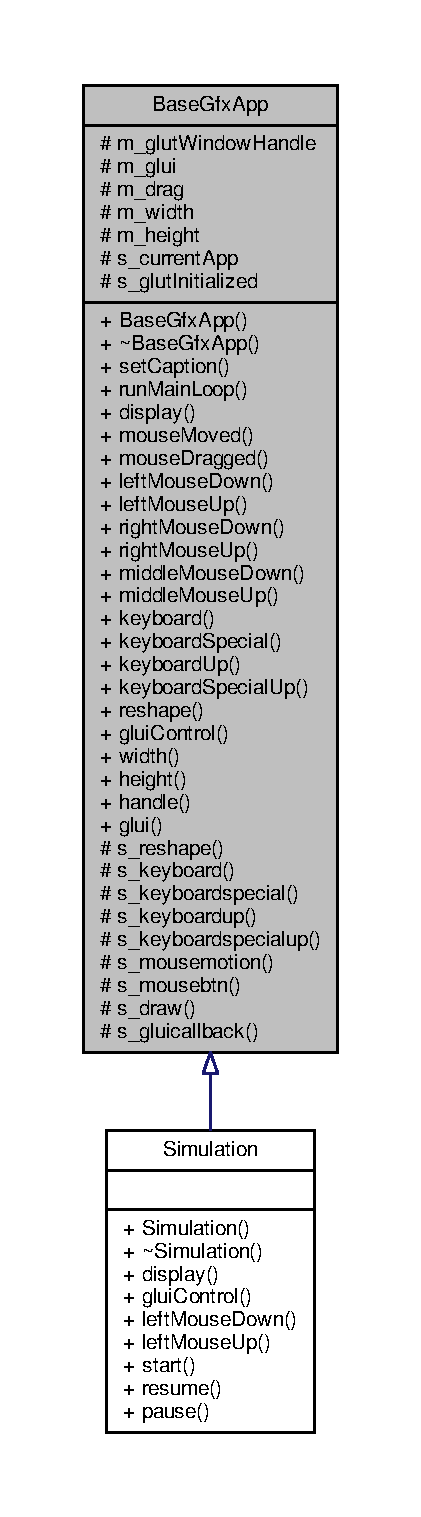
\includegraphics[height=550pt]{classBaseGfxApp__inherit__graph}
\end{center}
\end{figure}


Collaboration diagram for Base\-Gfx\-App\-:\nopagebreak
\begin{figure}[H]
\begin{center}
\leavevmode
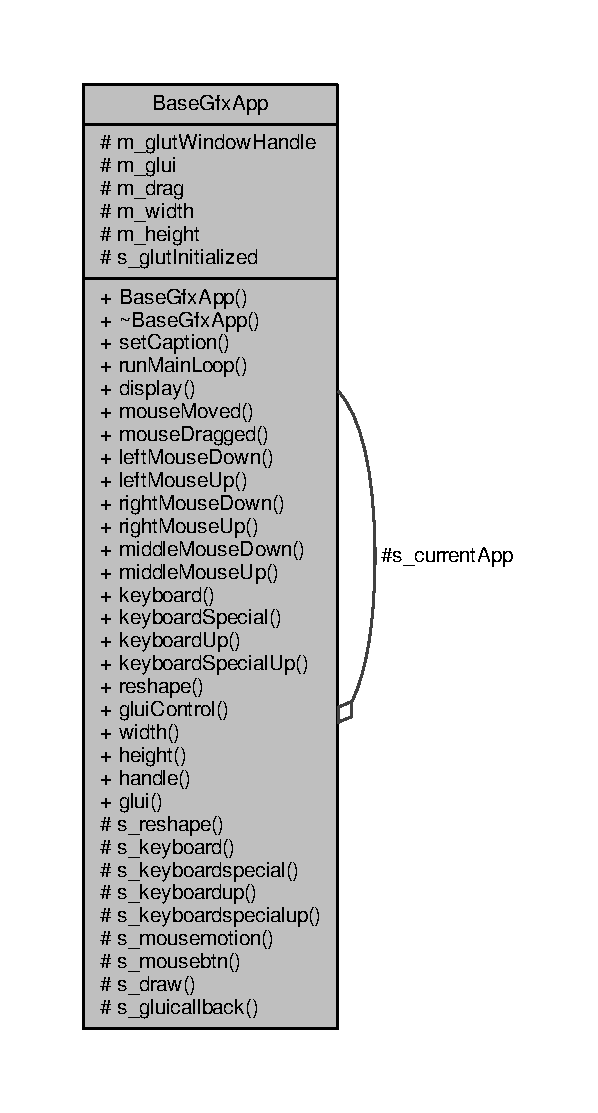
\includegraphics[width=287pt]{classBaseGfxApp__coll__graph}
\end{center}
\end{figure}
\subsection*{Public Member Functions}
\begin{DoxyCompactItemize}
\item 
\hypertarget{classBaseGfxApp_a534a4b5293a35947fdae3805a103541d}{{\bfseries Base\-Gfx\-App} (int argc, char $\ast$argv\mbox{[}$\,$\mbox{]}, int width, int height, int x, int y, int glut\-Flags, bool create\-G\-L\-U\-I\-Win, int glui\-Win\-X, int glui\-Win\-Y)}\label{classBaseGfxApp_a534a4b5293a35947fdae3805a103541d}

\item 
\hypertarget{classBaseGfxApp_a4b3b1a475b7f2babaf1b477c34b15fb1}{void {\bfseries set\-Caption} (const std\-::string \&caption)}\label{classBaseGfxApp_a4b3b1a475b7f2babaf1b477c34b15fb1}

\item 
\hypertarget{classBaseGfxApp_acda031916c00d56c2dc901e2653e3083}{void {\bfseries run\-Main\-Loop} ()}\label{classBaseGfxApp_acda031916c00d56c2dc901e2653e3083}

\item 
\hypertarget{classBaseGfxApp_ac8de2d5a955582547af5619b771b4d6d}{virtual void {\bfseries display} ()}\label{classBaseGfxApp_ac8de2d5a955582547af5619b771b4d6d}

\item 
\hypertarget{classBaseGfxApp_a0956b82d7fa58b623c498aea7073dbba}{virtual void {\bfseries mouse\-Moved} (int x, int y)}\label{classBaseGfxApp_a0956b82d7fa58b623c498aea7073dbba}

\item 
\hypertarget{classBaseGfxApp_abb23f716dd6612b3a72938e41525d338}{virtual void {\bfseries mouse\-Dragged} (int x, int y)}\label{classBaseGfxApp_abb23f716dd6612b3a72938e41525d338}

\item 
\hypertarget{classBaseGfxApp_aaaccf5a5e923a9465441a5ee712424a8}{virtual void {\bfseries left\-Mouse\-Down} (int x, int y)}\label{classBaseGfxApp_aaaccf5a5e923a9465441a5ee712424a8}

\item 
\hypertarget{classBaseGfxApp_a0a2961a932b02b2f9d7d0bb408f6fb51}{virtual void {\bfseries left\-Mouse\-Up} (int x, int y)}\label{classBaseGfxApp_a0a2961a932b02b2f9d7d0bb408f6fb51}

\item 
\hypertarget{classBaseGfxApp_afa87e6a71220945e41f0424e540125d9}{virtual void {\bfseries right\-Mouse\-Down} (int x, int y)}\label{classBaseGfxApp_afa87e6a71220945e41f0424e540125d9}

\item 
\hypertarget{classBaseGfxApp_a812643d563522a993457dd565c33f8f6}{virtual void {\bfseries right\-Mouse\-Up} (int x, int y)}\label{classBaseGfxApp_a812643d563522a993457dd565c33f8f6}

\item 
\hypertarget{classBaseGfxApp_a2c98cae9bb5ad1fb1832a6d4812670f8}{virtual void {\bfseries middle\-Mouse\-Down} (int x, int y)}\label{classBaseGfxApp_a2c98cae9bb5ad1fb1832a6d4812670f8}

\item 
\hypertarget{classBaseGfxApp_a00fc05e8d9629b72302b5adf014bdb0c}{virtual void {\bfseries middle\-Mouse\-Up} (int x, int y)}\label{classBaseGfxApp_a00fc05e8d9629b72302b5adf014bdb0c}

\item 
\hypertarget{classBaseGfxApp_a6d91e0cb7a3d48cad33956efe7eb36ca}{virtual void {\bfseries keyboard} (unsigned char c, int x, int y)}\label{classBaseGfxApp_a6d91e0cb7a3d48cad33956efe7eb36ca}

\item 
\hypertarget{classBaseGfxApp_a345566e62c9e4ec3705ec4d1c4c75f1f}{virtual void {\bfseries keyboard\-Special} (int key, int x, int y)}\label{classBaseGfxApp_a345566e62c9e4ec3705ec4d1c4c75f1f}

\item 
\hypertarget{classBaseGfxApp_acc4a40ce11edd6b6660a19cb4802a2bf}{virtual void {\bfseries keyboard\-Up} (unsigned char c, int x, int y)}\label{classBaseGfxApp_acc4a40ce11edd6b6660a19cb4802a2bf}

\item 
\hypertarget{classBaseGfxApp_afd14b435ff93b1e7f461cb8bd1a6fd59}{virtual void {\bfseries keyboard\-Special\-Up} (int key, int x, int y)}\label{classBaseGfxApp_afd14b435ff93b1e7f461cb8bd1a6fd59}

\item 
\hypertarget{classBaseGfxApp_a5d8d5d778a8aecd7f5f8e9c87f4c3d20}{virtual void {\bfseries reshape} (int width, int height)}\label{classBaseGfxApp_a5d8d5d778a8aecd7f5f8e9c87f4c3d20}

\item 
\hypertarget{classBaseGfxApp_a2978a7c358794c67df73b66776b2cef3}{virtual void {\bfseries glui\-Control} (int control\-I\-D)}\label{classBaseGfxApp_a2978a7c358794c67df73b66776b2cef3}

\item 
\hypertarget{classBaseGfxApp_ace089a1a94fb6bb0bc17e1b7fa48e05d}{int {\bfseries width} () const }\label{classBaseGfxApp_ace089a1a94fb6bb0bc17e1b7fa48e05d}

\item 
\hypertarget{classBaseGfxApp_aa253dbe16a20c40e0a1bf8ff942ceea3}{int {\bfseries height} () const }\label{classBaseGfxApp_aa253dbe16a20c40e0a1bf8ff942ceea3}

\item 
\hypertarget{classBaseGfxApp_ae9779f948eff6f45beec08091e98a803}{int {\bfseries handle} ()}\label{classBaseGfxApp_ae9779f948eff6f45beec08091e98a803}

\item 
\hypertarget{classBaseGfxApp_ac721a0fedce80308c5c0e5695016e95d}{G\-L\-U\-I $\ast$ {\bfseries glui} ()}\label{classBaseGfxApp_ac721a0fedce80308c5c0e5695016e95d}

\end{DoxyCompactItemize}
\subsection*{Static Protected Member Functions}
\begin{DoxyCompactItemize}
\item 
\hypertarget{classBaseGfxApp_a5fe6a77d37044cbe28647ed3391bbb7a}{static void {\bfseries s\-\_\-reshape} (int width, int height)}\label{classBaseGfxApp_a5fe6a77d37044cbe28647ed3391bbb7a}

\item 
\hypertarget{classBaseGfxApp_a52edb2569227319feb68779844e7d857}{static void {\bfseries s\-\_\-keyboard} (unsigned char c, int x, int y)}\label{classBaseGfxApp_a52edb2569227319feb68779844e7d857}

\item 
\hypertarget{classBaseGfxApp_a1e8d90a4faab60300ddf2a4ea9b83115}{static void {\bfseries s\-\_\-keyboardspecial} (int key, int x, int y)}\label{classBaseGfxApp_a1e8d90a4faab60300ddf2a4ea9b83115}

\item 
\hypertarget{classBaseGfxApp_aa1ca205af9d6cee33949f2e6adf4c923}{static void {\bfseries s\-\_\-keyboardup} (unsigned char c, int x, int y)}\label{classBaseGfxApp_aa1ca205af9d6cee33949f2e6adf4c923}

\item 
\hypertarget{classBaseGfxApp_a0e4dfe006f3cc9126c1cc8ad32784f75}{static void {\bfseries s\-\_\-keyboardspecialup} (int key, int x, int y)}\label{classBaseGfxApp_a0e4dfe006f3cc9126c1cc8ad32784f75}

\item 
\hypertarget{classBaseGfxApp_a5e640f2394f7e038d0dd2b469d5c2e24}{static void {\bfseries s\-\_\-mousemotion} (int x, int y)}\label{classBaseGfxApp_a5e640f2394f7e038d0dd2b469d5c2e24}

\item 
\hypertarget{classBaseGfxApp_a22dd953bfb75add9fd0f8f2f8be535c5}{static void {\bfseries s\-\_\-mousebtn} (int b, int s, int x, int y)}\label{classBaseGfxApp_a22dd953bfb75add9fd0f8f2f8be535c5}

\item 
\hypertarget{classBaseGfxApp_a58415c6151a2a80e1fe2eaa9919a4dab}{static void {\bfseries s\-\_\-draw} ()}\label{classBaseGfxApp_a58415c6151a2a80e1fe2eaa9919a4dab}

\item 
\hypertarget{classBaseGfxApp_ad4a963321f1147d68369225ab0c7f32f}{static void {\bfseries s\-\_\-gluicallback} (int control\-I\-D)}\label{classBaseGfxApp_ad4a963321f1147d68369225ab0c7f32f}

\end{DoxyCompactItemize}
\subsection*{Protected Attributes}
\begin{DoxyCompactItemize}
\item 
int \hyperlink{classBaseGfxApp_ad8697d6fdd10e6f336c3a662016b4fa7}{m\-\_\-glut\-Window\-Handle}
\item 
\hypertarget{classBaseGfxApp_a6eb1673b80283727221da2242211af1d}{G\-L\-U\-I $\ast$ {\bfseries m\-\_\-glui}}\label{classBaseGfxApp_a6eb1673b80283727221da2242211af1d}

\item 
\hypertarget{classBaseGfxApp_a2e70a389224f8affe7c137f7e20dc8c1}{bool {\bfseries m\-\_\-drag}}\label{classBaseGfxApp_a2e70a389224f8affe7c137f7e20dc8c1}

\item 
\hypertarget{classBaseGfxApp_a7e5ef1c8f25fe081b4a1fd4ce6a96e07}{int {\bfseries m\-\_\-width}}\label{classBaseGfxApp_a7e5ef1c8f25fe081b4a1fd4ce6a96e07}

\item 
\hypertarget{classBaseGfxApp_ac078e4fc20b5c2fe0c744966b850b412}{int {\bfseries m\-\_\-height}}\label{classBaseGfxApp_ac078e4fc20b5c2fe0c744966b850b412}

\end{DoxyCompactItemize}
\subsection*{Static Protected Attributes}
\begin{DoxyCompactItemize}
\item 
static \hyperlink{classBaseGfxApp}{Base\-Gfx\-App} $\ast$ \hyperlink{classBaseGfxApp_a65ba89b98af31e2649a0546631931000}{s\-\_\-current\-App} = N\-U\-L\-L
\item 
static bool \hyperlink{classBaseGfxApp_afa4690383ea27713016ef75b9fb1e42f}{s\-\_\-glut\-Initialized} = false
\end{DoxyCompactItemize}


\subsection{Member Data Documentation}
\hypertarget{classBaseGfxApp_ad8697d6fdd10e6f336c3a662016b4fa7}{\index{Base\-Gfx\-App@{Base\-Gfx\-App}!m\-\_\-glut\-Window\-Handle@{m\-\_\-glut\-Window\-Handle}}
\index{m\-\_\-glut\-Window\-Handle@{m\-\_\-glut\-Window\-Handle}!BaseGfxApp@{Base\-Gfx\-App}}
\subsubsection[{m\-\_\-glut\-Window\-Handle}]{\setlength{\rightskip}{0pt plus 5cm}int Base\-Gfx\-App\-::m\-\_\-glut\-Window\-Handle\hspace{0.3cm}{\ttfamily [protected]}}}\label{classBaseGfxApp_ad8697d6fdd10e6f336c3a662016b4fa7}
Underlying glut window handle \hypertarget{classBaseGfxApp_a65ba89b98af31e2649a0546631931000}{\index{Base\-Gfx\-App@{Base\-Gfx\-App}!s\-\_\-current\-App@{s\-\_\-current\-App}}
\index{s\-\_\-current\-App@{s\-\_\-current\-App}!BaseGfxApp@{Base\-Gfx\-App}}
\subsubsection[{s\-\_\-current\-App}]{\setlength{\rightskip}{0pt plus 5cm}{\bf Base\-Gfx\-App} $\ast$ Base\-Gfx\-App\-::s\-\_\-current\-App = N\-U\-L\-L\hspace{0.3cm}{\ttfamily [static]}, {\ttfamily [protected]}}}\label{classBaseGfxApp_a65ba89b98af31e2649a0546631931000}
G\-L\-U\-T and G\-L\-U\-I event callbacks are sent to the current window/app. Right now, there is only one window anyway (not counting the G\-L\-U\-I U\-I window.. in the future could be extended to support more windows. In any case, some structure like this is always needed when using glut with C++, since the glut callbacks must be either global or static functions. \hypertarget{classBaseGfxApp_afa4690383ea27713016ef75b9fb1e42f}{\index{Base\-Gfx\-App@{Base\-Gfx\-App}!s\-\_\-glut\-Initialized@{s\-\_\-glut\-Initialized}}
\index{s\-\_\-glut\-Initialized@{s\-\_\-glut\-Initialized}!BaseGfxApp@{Base\-Gfx\-App}}
\subsubsection[{s\-\_\-glut\-Initialized}]{\setlength{\rightskip}{0pt plus 5cm}bool Base\-Gfx\-App\-::s\-\_\-glut\-Initialized = false\hspace{0.3cm}{\ttfamily [static]}, {\ttfamily [protected]}}}\label{classBaseGfxApp_afa4690383ea27713016ef75b9fb1e42f}
Has glut\-Init been called? (only allowed once per program) 

The documentation for this class was generated from the following files\-:\begin{DoxyCompactItemize}
\item 
\hyperlink{BaseGfxApp_8h}{Base\-Gfx\-App.\-h}\item 
Base\-Gfx\-App.\-cpp\end{DoxyCompactItemize}

\hypertarget{classEnvironmentClass}{\section{Environment\-Class Class Reference}
\label{classEnvironmentClass}\index{Environment\-Class@{Environment\-Class}}
}


Collaboration diagram for Environment\-Class\-:
\nopagebreak
\begin{figure}[H]
\begin{center}
\leavevmode
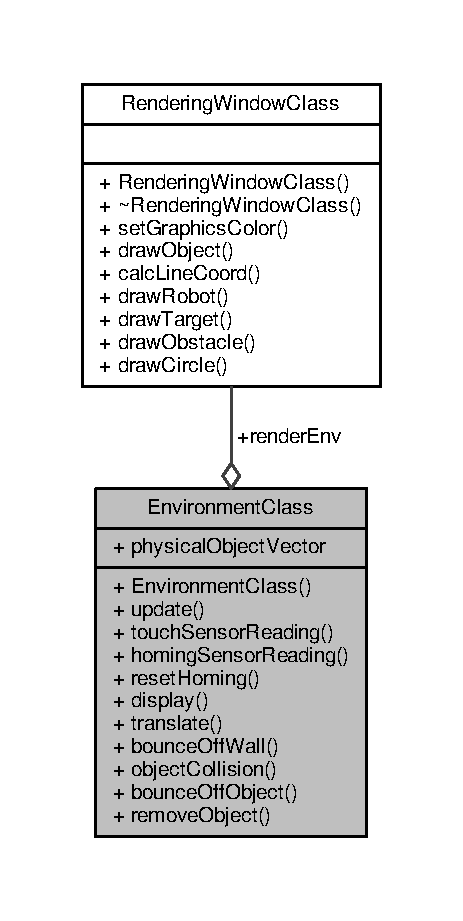
\includegraphics[width=222pt]{classEnvironmentClass__coll__graph}
\end{center}
\end{figure}
\subsection*{Public Member Functions}
\begin{DoxyCompactItemize}
\item 
\hypertarget{classEnvironmentClass_aa69ad01551a79f7326f005709061ff31}{\hyperlink{classEnvironmentClass_aa69ad01551a79f7326f005709061ff31}{Environment\-Class} ()}\label{classEnvironmentClass_aa69ad01551a79f7326f005709061ff31}

\begin{DoxyCompactList}\small\item\em default constructor for \hyperlink{classEnvironmentClass}{Environment\-Class} \end{DoxyCompactList}\item 
void \hyperlink{classEnvironmentClass_a7d992b6ef4e8b95542af1ae775be988a}{update} (double elapsed\-Time)
\begin{DoxyCompactList}\small\item\em updates each object by calling move, then setting position \end{DoxyCompactList}\item 
int \hyperlink{classEnvironmentClass_a2c810b4fe1f93852659686ae392b0a8a}{touch\-Sensor\-Reading} (\hyperlink{classPhysicalObjectClass}{Physical\-Object\-Class} $\ast$object)
\begin{DoxyCompactList}\small\item\em Collision detection. \end{DoxyCompactList}\item 
void \hyperlink{classEnvironmentClass_a47912774c37cc6185c0b409e4b7789e3}{homing\-Sensor\-Reading} (\hyperlink{classRobotClass}{Robot\-Class} $\ast$robot, \hyperlink{classTargetClass}{Target\-Class} $\ast$target)
\begin{DoxyCompactList}\small\item\em Determines robot to target orientation. \end{DoxyCompactList}\item 
void \hyperlink{classEnvironmentClass_a7dd5a652634672bbaf5c00e214add9f6}{reset\-Homing} (\hyperlink{classPhysicalObjectClass}{Physical\-Object\-Class} $\ast$object)
\begin{DoxyCompactList}\small\item\em Determines robot's corresponding target. \end{DoxyCompactList}\item 
void \hyperlink{classEnvironmentClass_a862919dd05c8ec626360f11b809bd6ae}{display} ()
\begin{DoxyCompactList}\small\item\em Draw and displays objects and environment. \end{DoxyCompactList}\item 
void \hyperlink{classEnvironmentClass_a0fa52a8dd735412f9d46f4e2499e8108}{translate} (\hyperlink{classPhysicalObjectClass}{Physical\-Object\-Class} $\ast$object, double elapsed\-Time)
\begin{DoxyCompactList}\small\item\em Moves the input object. \end{DoxyCompactList}\item 
void \hyperlink{classEnvironmentClass_a2073fafc0218848ea81d21138ea702b7}{bounce\-Off\-Wall} (\hyperlink{classPhysicalObjectClass}{Physical\-Object\-Class} $\ast$object)
\begin{DoxyCompactList}\small\item\em Performs wall collision movement. \end{DoxyCompactList}\item 
void \hyperlink{classEnvironmentClass_a6ce1e78294fb94ac1fc27cf3ef1f0419}{object\-Collision} (\hyperlink{classPhysicalObjectClass}{Physical\-Object\-Class} $\ast$current\-Object, \hyperlink{classPhysicalObjectClass}{Physical\-Object\-Class} $\ast$hit\-Object, double elapsed\-Time)
\begin{DoxyCompactList}\small\item\em Object collision management. \end{DoxyCompactList}\item 
void \hyperlink{classEnvironmentClass_aa57351175592327c191e0d84ef2be6e3}{bounce\-Off\-Object} (\hyperlink{classPhysicalObjectClass}{Physical\-Object\-Class} $\ast$current\-Object, \hyperlink{classPhysicalObjectClass}{Physical\-Object\-Class} $\ast$hit\-Object)
\begin{DoxyCompactList}\small\item\em Performs object collision movement. \end{DoxyCompactList}\item 
void \hyperlink{classEnvironmentClass_a564160db6ba48653b24b3a42ce9d2d58}{remove\-Object} (\hyperlink{classPhysicalObjectClass}{Physical\-Object\-Class} $\ast$object)
\begin{DoxyCompactList}\small\item\em Removes the object from the simulation. \end{DoxyCompactList}\end{DoxyCompactItemize}
\subsection*{Public Attributes}
\begin{DoxyCompactItemize}
\item 
\hypertarget{classEnvironmentClass_a3735bf3dc818a03984620368f196b1d0}{std\-::vector\\*
$<$ \hyperlink{classPhysicalObjectClass}{Physical\-Object\-Class} $\ast$ $>$ {\bfseries physical\-Object\-Vector}}\label{classEnvironmentClass_a3735bf3dc818a03984620368f196b1d0}

\item 
\hypertarget{classEnvironmentClass_a403bb85973a4db56e0163686147dae8b}{\hyperlink{classRenderingWindowClass}{Rendering\-Window\-Class} $\ast$ {\bfseries render\-Env}}\label{classEnvironmentClass_a403bb85973a4db56e0163686147dae8b}

\end{DoxyCompactItemize}


\subsection{Member Function Documentation}
\hypertarget{classEnvironmentClass_aa57351175592327c191e0d84ef2be6e3}{\index{Environment\-Class@{Environment\-Class}!bounce\-Off\-Object@{bounce\-Off\-Object}}
\index{bounce\-Off\-Object@{bounce\-Off\-Object}!EnvironmentClass@{Environment\-Class}}
\subsubsection[{bounce\-Off\-Object}]{\setlength{\rightskip}{0pt plus 5cm}void Environment\-Class\-::bounce\-Off\-Object (
\begin{DoxyParamCaption}
\item[{{\bf Physical\-Object\-Class} $\ast$}]{current\-Object, }
\item[{{\bf Physical\-Object\-Class} $\ast$}]{hit\-Object}
\end{DoxyParamCaption}
)}}\label{classEnvironmentClass_aa57351175592327c191e0d84ef2be6e3}


Performs object collision movement. 

This function sets the new orientations of the objects that are colliding to be 90 degrees away from each other.


\begin{DoxyParams}{Parameters}
{\em current\-Object} & the object making the collision \\
\hline
{\em hit\-Object} & the object being collided into \\
\hline
\end{DoxyParams}
\hypertarget{classEnvironmentClass_a2073fafc0218848ea81d21138ea702b7}{\index{Environment\-Class@{Environment\-Class}!bounce\-Off\-Wall@{bounce\-Off\-Wall}}
\index{bounce\-Off\-Wall@{bounce\-Off\-Wall}!EnvironmentClass@{Environment\-Class}}
\subsubsection[{bounce\-Off\-Wall}]{\setlength{\rightskip}{0pt plus 5cm}void Environment\-Class\-::bounce\-Off\-Wall (
\begin{DoxyParamCaption}
\item[{{\bf Physical\-Object\-Class} $\ast$}]{object}
\end{DoxyParamCaption}
)}}\label{classEnvironmentClass_a2073fafc0218848ea81d21138ea702b7}


Performs wall collision movement. 

This function determines which wall the object is colliding with and which direction it is coming from, and then subsequently changes its orientation to be 90 degrees away from the wall and translated inwards one pixel to remain in the window.


\begin{DoxyParams}{Parameters}
{\em object} & the object that is bouncing off the wall \\
\hline
\end{DoxyParams}
\hypertarget{classEnvironmentClass_a862919dd05c8ec626360f11b809bd6ae}{\index{Environment\-Class@{Environment\-Class}!display@{display}}
\index{display@{display}!EnvironmentClass@{Environment\-Class}}
\subsubsection[{display}]{\setlength{\rightskip}{0pt plus 5cm}void Environment\-Class\-::display (
\begin{DoxyParamCaption}
{}
\end{DoxyParamCaption}
)}}\label{classEnvironmentClass_a862919dd05c8ec626360f11b809bd6ae}


Draw and displays objects and environment. 

This function is constantly called from simulation. It displays and draws all the objects and calls the update function and effectively sets up the environment. \hypertarget{classEnvironmentClass_a47912774c37cc6185c0b409e4b7789e3}{\index{Environment\-Class@{Environment\-Class}!homing\-Sensor\-Reading@{homing\-Sensor\-Reading}}
\index{homing\-Sensor\-Reading@{homing\-Sensor\-Reading}!EnvironmentClass@{Environment\-Class}}
\subsubsection[{homing\-Sensor\-Reading}]{\setlength{\rightskip}{0pt plus 5cm}void Environment\-Class\-::homing\-Sensor\-Reading (
\begin{DoxyParamCaption}
\item[{{\bf Robot\-Class} $\ast$}]{robot, }
\item[{{\bf Target\-Class} $\ast$}]{target}
\end{DoxyParamCaption}
)}}\label{classEnvironmentClass_a47912774c37cc6185c0b409e4b7789e3}


Determines robot to target orientation. 

This function takes in a robot-\/target pair and calculates the orientation that points to the target, and then it sets the robot's orientation to that.


\begin{DoxyParams}{Parameters}
{\em robot} & the robot that is trying to home in on target \\
\hline
{\em target} & the target that is being homed in on by robot \\
\hline
\end{DoxyParams}
\hypertarget{classEnvironmentClass_a6ce1e78294fb94ac1fc27cf3ef1f0419}{\index{Environment\-Class@{Environment\-Class}!object\-Collision@{object\-Collision}}
\index{object\-Collision@{object\-Collision}!EnvironmentClass@{Environment\-Class}}
\subsubsection[{object\-Collision}]{\setlength{\rightskip}{0pt plus 5cm}void Environment\-Class\-::object\-Collision (
\begin{DoxyParamCaption}
\item[{{\bf Physical\-Object\-Class} $\ast$}]{current\-Object, }
\item[{{\bf Physical\-Object\-Class} $\ast$}]{hit\-Object, }
\item[{double}]{elapsed\-Time}
\end{DoxyParamCaption}
)}}\label{classEnvironmentClass_a6ce1e78294fb94ac1fc27cf3ef1f0419}


Object collision management. 

This function determines what type of object the current\-Object is colliding into and then subsequently determines its corresponding behavior.


\begin{DoxyParams}{Parameters}
{\em current\-Object} & the object making the collision \\
\hline
{\em hit\-Object} & the object being collided into \\
\hline
{\em elapsed\-Time} & the amount of time passed \\
\hline
\end{DoxyParams}
\hypertarget{classEnvironmentClass_a564160db6ba48653b24b3a42ce9d2d58}{\index{Environment\-Class@{Environment\-Class}!remove\-Object@{remove\-Object}}
\index{remove\-Object@{remove\-Object}!EnvironmentClass@{Environment\-Class}}
\subsubsection[{remove\-Object}]{\setlength{\rightskip}{0pt plus 5cm}void Environment\-Class\-::remove\-Object (
\begin{DoxyParamCaption}
\item[{{\bf Physical\-Object\-Class} $\ast$}]{object}
\end{DoxyParamCaption}
)}}\label{classEnvironmentClass_a564160db6ba48653b24b3a42ce9d2d58}


Removes the object from the simulation. 

This function \char`\"{}removes\char`\"{} the input object from the simulation by setting the should\-Be\-Drawn attribute to 0 and moving the object off screen.


\begin{DoxyParams}{Parameters}
{\em object} & the object that needs removing \\
\hline
\end{DoxyParams}
\hypertarget{classEnvironmentClass_a7dd5a652634672bbaf5c00e214add9f6}{\index{Environment\-Class@{Environment\-Class}!reset\-Homing@{reset\-Homing}}
\index{reset\-Homing@{reset\-Homing}!EnvironmentClass@{Environment\-Class}}
\subsubsection[{reset\-Homing}]{\setlength{\rightskip}{0pt plus 5cm}void Environment\-Class\-::reset\-Homing (
\begin{DoxyParamCaption}
\item[{{\bf Physical\-Object\-Class} $\ast$}]{object}
\end{DoxyParamCaption}
)}}\label{classEnvironmentClass_a7dd5a652634672bbaf5c00e214add9f6}


Determines robot's corresponding target. 

This function takes in a robot type object, finds its corresponding target, and calls homing\-Sensor\-Reading with these two objects. This essentially makes sure that the robot will be homing in on its own target and not different one.


\begin{DoxyParams}{Parameters}
{\em object} & whichever robot is requesting homing sensor info \\
\hline
\end{DoxyParams}
\hypertarget{classEnvironmentClass_a2c810b4fe1f93852659686ae392b0a8a}{\index{Environment\-Class@{Environment\-Class}!touch\-Sensor\-Reading@{touch\-Sensor\-Reading}}
\index{touch\-Sensor\-Reading@{touch\-Sensor\-Reading}!EnvironmentClass@{Environment\-Class}}
\subsubsection[{touch\-Sensor\-Reading}]{\setlength{\rightskip}{0pt plus 5cm}int Environment\-Class\-::touch\-Sensor\-Reading (
\begin{DoxyParamCaption}
\item[{{\bf Physical\-Object\-Class} $\ast$}]{object}
\end{DoxyParamCaption}
)}}\label{classEnvironmentClass_a2c810b4fe1f93852659686ae392b0a8a}


Collision detection. 

This function takes in an object and checks if that object is colliding with another object or a wall. It returns -\/1 if the object is not colliding with anything, -\/2 if it is colliding with a wall, or the index of the object it is colliding with.


\begin{DoxyParams}{Parameters}
{\em object} & whichever object is requesting touch sensor information \\
\hline
\end{DoxyParams}
\begin{DoxyReturn}{Returns}
-\/1 if the object is not colliding with anything -\/2 if the object is colliding with a wall index of the object the input object is colliding with 
\end{DoxyReturn}
\hypertarget{classEnvironmentClass_a0fa52a8dd735412f9d46f4e2499e8108}{\index{Environment\-Class@{Environment\-Class}!translate@{translate}}
\index{translate@{translate}!EnvironmentClass@{Environment\-Class}}
\subsubsection[{translate}]{\setlength{\rightskip}{0pt plus 5cm}void Environment\-Class\-::translate (
\begin{DoxyParamCaption}
\item[{{\bf Physical\-Object\-Class} $\ast$}]{object, }
\item[{double}]{elapsed\-Time}
\end{DoxyParamCaption}
)}}\label{classEnvironmentClass_a0fa52a8dd735412f9d46f4e2499e8108}


Moves the input object. 

This function resets the location of the input object based on its speed, original location, orientation, and elapsed time.


\begin{DoxyParams}{Parameters}
{\em object} & the object being translating \\
\hline
{\em elapsed\-Time} & the amount of time passed \\
\hline
\end{DoxyParams}
\hypertarget{classEnvironmentClass_a7d992b6ef4e8b95542af1ae775be988a}{\index{Environment\-Class@{Environment\-Class}!update@{update}}
\index{update@{update}!EnvironmentClass@{Environment\-Class}}
\subsubsection[{update}]{\setlength{\rightskip}{0pt plus 5cm}void Environment\-Class\-::update (
\begin{DoxyParamCaption}
\item[{double}]{elapsed\-Time}
\end{DoxyParamCaption}
)}}\label{classEnvironmentClass_a7d992b6ef4e8b95542af1ae775be988a}


updates each object by calling move, then setting position 

This function takes an one argument, elapsed\-Time, and iterates through the physical\-Objects array, calling move each time. Move then returns an double\mbox{[}2\mbox{]} array containing the direction and magnitude of movement. Based on which coordinate the object currently is in, it sets the object's new position.


\begin{DoxyParams}{Parameters}
{\em elapsed\-Time} & the amount of time passed \\
\hline
\end{DoxyParams}


The documentation for this class was generated from the following files\-:\begin{DoxyCompactItemize}
\item 
\hyperlink{EnvironmentClass_8h}{Environment\-Class.\-h}\item 
\hyperlink{EnvironmentClass_8cpp}{Environment\-Class.\-cpp}\end{DoxyCompactItemize}

\hypertarget{classObstacleClass}{\section{Obstacle\-Class Class Reference}
\label{classObstacleClass}\index{Obstacle\-Class@{Obstacle\-Class}}
}


Inheritance diagram for Obstacle\-Class\-:
\nopagebreak
\begin{figure}[H]
\begin{center}
\leavevmode
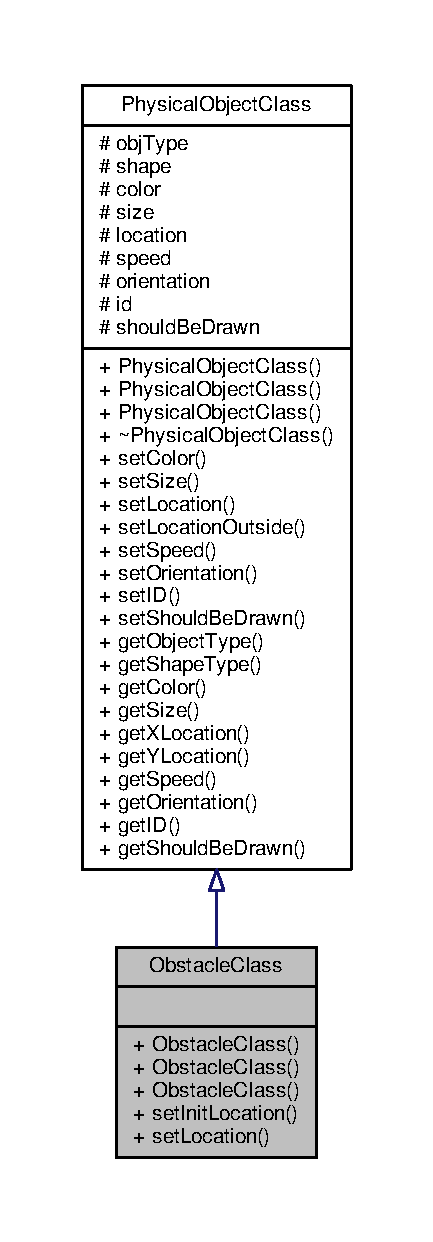
\includegraphics[height=550pt]{classObstacleClass__inherit__graph}
\end{center}
\end{figure}


Collaboration diagram for Obstacle\-Class\-:
\nopagebreak
\begin{figure}[H]
\begin{center}
\leavevmode
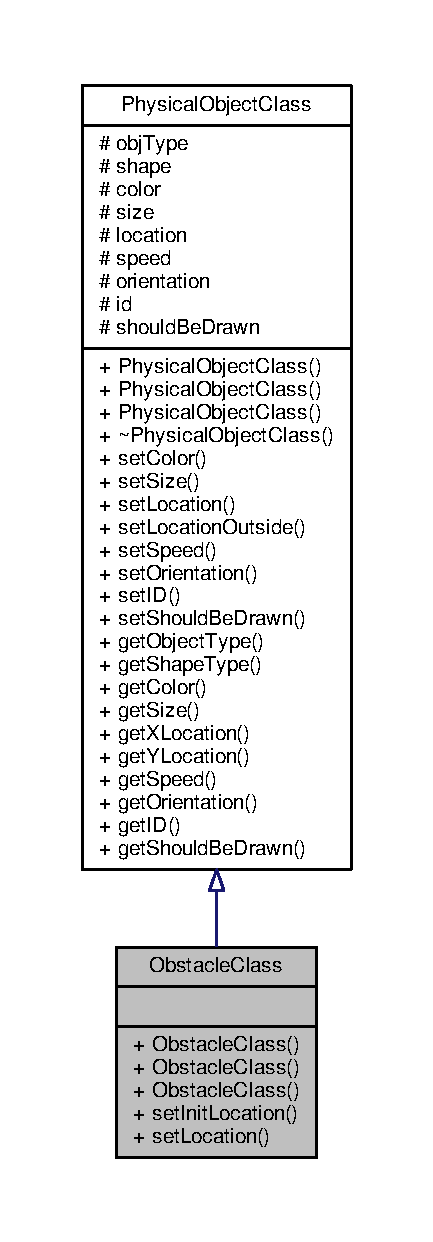
\includegraphics[height=550pt]{classObstacleClass__coll__graph}
\end{center}
\end{figure}
\subsection*{Public Member Functions}
\begin{DoxyCompactItemize}
\item 
\hyperlink{classObstacleClass_a7fa2d44335187a92e7a175e70963afd1}{Obstacle\-Class} ()
\begin{DoxyCompactList}\small\item\em default Obstacle constructor \end{DoxyCompactList}\item 
\hyperlink{classObstacleClass_aff7cabe763e79d642912d7f95a681a52}{Obstacle\-Class} (\hyperlink{PhysicalObjectClass_8h_a5a4538eeab397888d88a4eefcc5a1345}{Shape\-Type} shape\-In, int size\-In)
\begin{DoxyCompactList}\small\item\em obstacle constructor with two parameters \end{DoxyCompactList}\item 
\hyperlink{classObstacleClass_a019600b458c09a3190d637638fd24e8d}{Obstacle\-Class} (\hyperlink{PhysicalObjectClass_8h_a5a4538eeab397888d88a4eefcc5a1345}{Shape\-Type} shape\-In, int size\-In, double x, double y)
\begin{DoxyCompactList}\small\item\em obstacle constructor with 4 paramters \end{DoxyCompactList}\item 
void \hyperlink{classObstacleClass_a7441fc7bc4c504dad86558b4f4314443}{set\-Init\-Location} (double x, double y)
\begin{DoxyCompactList}\small\item\em Sets the initial obstacle location. \end{DoxyCompactList}\item 
void \hyperlink{classObstacleClass_ab405faf368836ef45a42fb4f7084631e}{set\-Location} (double x, double y)
\begin{DoxyCompactList}\small\item\em sets object Position \end{DoxyCompactList}\end{DoxyCompactItemize}
\subsection*{Additional Inherited Members}


\subsection{Constructor \& Destructor Documentation}
\hypertarget{classObstacleClass_a7fa2d44335187a92e7a175e70963afd1}{\index{Obstacle\-Class@{Obstacle\-Class}!Obstacle\-Class@{Obstacle\-Class}}
\index{Obstacle\-Class@{Obstacle\-Class}!ObstacleClass@{Obstacle\-Class}}
\subsubsection[{Obstacle\-Class}]{\setlength{\rightskip}{0pt plus 5cm}Obstacle\-Class\-::\-Obstacle\-Class (
\begin{DoxyParamCaption}
{}
\end{DoxyParamCaption}
)}}\label{classObstacleClass_a7fa2d44335187a92e7a175e70963afd1}


default Obstacle constructor 

This constructor creates an circle with size 5 and a random location \hypertarget{classObstacleClass_aff7cabe763e79d642912d7f95a681a52}{\index{Obstacle\-Class@{Obstacle\-Class}!Obstacle\-Class@{Obstacle\-Class}}
\index{Obstacle\-Class@{Obstacle\-Class}!ObstacleClass@{Obstacle\-Class}}
\subsubsection[{Obstacle\-Class}]{\setlength{\rightskip}{0pt plus 5cm}Obstacle\-Class\-::\-Obstacle\-Class (
\begin{DoxyParamCaption}
\item[{{\bf Shape\-Type}}]{shape\-In, }
\item[{int}]{size\-In}
\end{DoxyParamCaption}
)}}\label{classObstacleClass_aff7cabe763e79d642912d7f95a681a52}


obstacle constructor with two parameters 

This constructor creates an obstacle of type shape\-In with size size\-In \hypertarget{classObstacleClass_a019600b458c09a3190d637638fd24e8d}{\index{Obstacle\-Class@{Obstacle\-Class}!Obstacle\-Class@{Obstacle\-Class}}
\index{Obstacle\-Class@{Obstacle\-Class}!ObstacleClass@{Obstacle\-Class}}
\subsubsection[{Obstacle\-Class}]{\setlength{\rightskip}{0pt plus 5cm}Obstacle\-Class\-::\-Obstacle\-Class (
\begin{DoxyParamCaption}
\item[{{\bf Shape\-Type}}]{shape\-In, }
\item[{int}]{size\-In, }
\item[{double}]{x, }
\item[{double}]{y}
\end{DoxyParamCaption}
)}}\label{classObstacleClass_a019600b458c09a3190d637638fd24e8d}


obstacle constructor with 4 paramters 

This constructor creates an obstacle of type shape\-In with size size\-In, x-\/position x, and y position y 
\begin{DoxyParams}{Parameters}
{\em shape\-In} & Enum shape \\
\hline
{\em size\-In} & integer size of shape \\
\hline
{\em x} & integer x coordinate (in pixels) \\
\hline
{\em y} & integer y coordinate (in pixels) \\
\hline
\end{DoxyParams}


\subsection{Member Function Documentation}
\hypertarget{classObstacleClass_a7441fc7bc4c504dad86558b4f4314443}{\index{Obstacle\-Class@{Obstacle\-Class}!set\-Init\-Location@{set\-Init\-Location}}
\index{set\-Init\-Location@{set\-Init\-Location}!ObstacleClass@{Obstacle\-Class}}
\subsubsection[{set\-Init\-Location}]{\setlength{\rightskip}{0pt plus 5cm}void Obstacle\-Class\-::set\-Init\-Location (
\begin{DoxyParamCaption}
\item[{double}]{x, }
\item[{double}]{y}
\end{DoxyParamCaption}
)}}\label{classObstacleClass_a7441fc7bc4c504dad86558b4f4314443}


Sets the initial obstacle location. 

Sets the initial obstacle location, ensuring that the obstacle will not overlap with any other objects


\begin{DoxyParams}{Parameters}
{\em x} & x double location of the obstacle \\
\hline
{\em y} & y double location of the obstacle \\
\hline
\end{DoxyParams}
\hypertarget{classObstacleClass_ab405faf368836ef45a42fb4f7084631e}{\index{Obstacle\-Class@{Obstacle\-Class}!set\-Location@{set\-Location}}
\index{set\-Location@{set\-Location}!ObstacleClass@{Obstacle\-Class}}
\subsubsection[{set\-Location}]{\setlength{\rightskip}{0pt plus 5cm}void Obstacle\-Class\-::set\-Location (
\begin{DoxyParamCaption}
\item[{double}]{x, }
\item[{double}]{y}
\end{DoxyParamCaption}
)\hspace{0.3cm}{\ttfamily [virtual]}}}\label{classObstacleClass_ab405faf368836ef45a42fb4f7084631e}


sets object Position 

This function sets the obstacle's x-\/ and y-\/positions to the integer input from the user


\begin{DoxyParams}{Parameters}
{\em x,y} & \\
\hline
\end{DoxyParams}


Reimplemented from \hyperlink{classPhysicalObjectClass_a3f9833aa04aa438de63b82fc761910ba}{Physical\-Object\-Class}.



The documentation for this class was generated from the following files\-:\begin{DoxyCompactItemize}
\item 
\hyperlink{ObstacleClass_8h}{Obstacle\-Class.\-h}\item 
\hyperlink{ObstacleClass_8cpp}{Obstacle\-Class.\-cpp}\end{DoxyCompactItemize}

\input{classObstacleClassTests}
\hypertarget{classPhysicalObjectClass}{\section{Physical\-Object\-Class Class Reference}
\label{classPhysicalObjectClass}\index{Physical\-Object\-Class@{Physical\-Object\-Class}}
}


Inheritance diagram for Physical\-Object\-Class\-:
\nopagebreak
\begin{figure}[H]
\begin{center}
\leavevmode
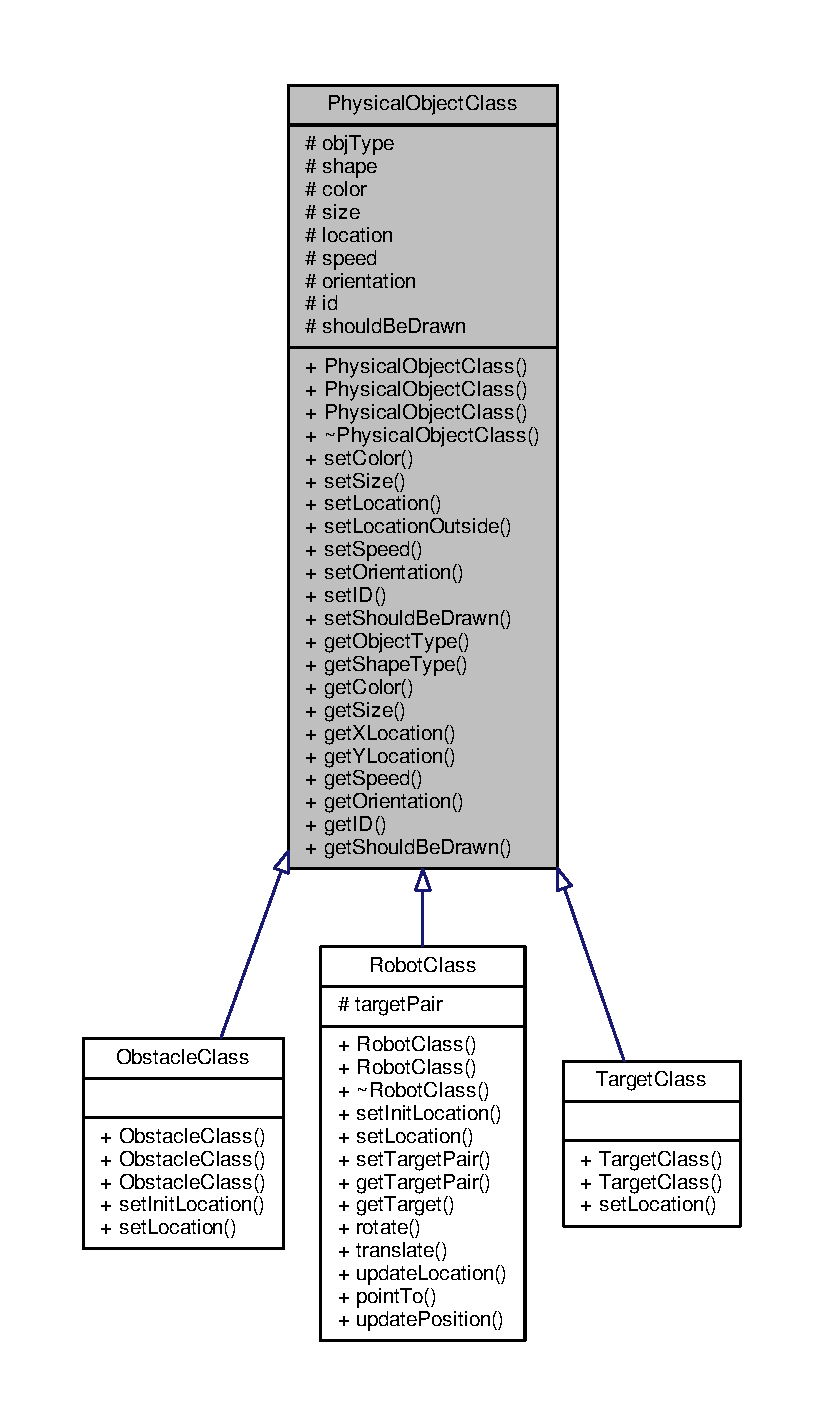
\includegraphics[height=550pt]{classPhysicalObjectClass__inherit__graph}
\end{center}
\end{figure}


Collaboration diagram for Physical\-Object\-Class\-:
\nopagebreak
\begin{figure}[H]
\begin{center}
\leavevmode
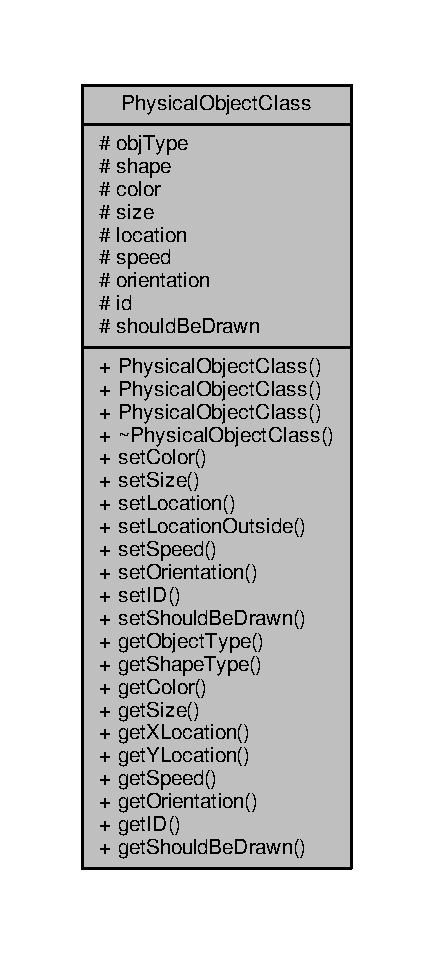
\includegraphics[width=208pt]{classPhysicalObjectClass__coll__graph}
\end{center}
\end{figure}
\subsection*{Public Member Functions}
\begin{DoxyCompactItemize}
\item 
\hyperlink{classPhysicalObjectClass_a960979388739197bbf20ac18d08d7021}{Physical\-Object\-Class} ()
\begin{DoxyCompactList}\small\item\em Default constructor for \hyperlink{classPhysicalObjectClass}{Physical\-Object\-Class}. \end{DoxyCompactList}\item 
\hypertarget{classPhysicalObjectClass_a7cdfb22cf10eab196c05058891d15911}{{\bfseries Physical\-Object\-Class} (double x, double y, int size\-In, double speed\-In)}\label{classPhysicalObjectClass_a7cdfb22cf10eab196c05058891d15911}

\item 
\hypertarget{classPhysicalObjectClass_a65c7fba02b87fbf45ff775cc3225dba6}{{\bfseries Physical\-Object\-Class} (\hyperlink{PhysicalObjectClass_8h_a842c5e2e69277690b064bf363c017980}{Object\-Type} obj\-Type\-In, \hyperlink{PhysicalObjectClass_8h_a5a4538eeab397888d88a4eefcc5a1345}{Shape\-Type} obj\-Shape\-In, char color\-In, double x, double y, int size\-In, double speed\-In, int orientation\-In, int id\-In, int sbd\-In)}\label{classPhysicalObjectClass_a65c7fba02b87fbf45ff775cc3225dba6}

\item 
\hypertarget{classPhysicalObjectClass_a97db381b4e2e357eeb8aeeb580d0b7bd}{\hyperlink{classPhysicalObjectClass_a97db381b4e2e357eeb8aeeb580d0b7bd}{$\sim$\-Physical\-Object\-Class} ()}\label{classPhysicalObjectClass_a97db381b4e2e357eeb8aeeb580d0b7bd}

\begin{DoxyCompactList}\small\item\em Default destructor for \hyperlink{classPhysicalObjectClass}{Physical\-Object\-Class}. \end{DoxyCompactList}\item 
void \hyperlink{classPhysicalObjectClass_aed8b6e0511dd981e8161eabfc6705be1}{set\-Color} (char color\-In)
\begin{DoxyCompactList}\small\item\em Set the Physical\-Object color. \end{DoxyCompactList}\item 
void \hyperlink{classPhysicalObjectClass_a02c35b30ac5f7c02d006ec0c008d7280}{set\-Size} (int size\-In)
\begin{DoxyCompactList}\small\item\em Set the Physical\-Object size. \end{DoxyCompactList}\item 
virtual void \hyperlink{classPhysicalObjectClass_a3f9833aa04aa438de63b82fc761910ba}{set\-Location} (double x, double y)
\begin{DoxyCompactList}\small\item\em Set the Physical\-Object location. \end{DoxyCompactList}\item 
void \hyperlink{classPhysicalObjectClass_ad80f075cef71fd42587695936a5808fa}{set\-Location\-Outside} ()
\begin{DoxyCompactList}\small\item\em Set the Physical\-Object location outside of the G\-L\-U\-T window. \end{DoxyCompactList}\item 
void \hyperlink{classPhysicalObjectClass_ab8315565f193dd26f7069480d820a7c9}{set\-Speed} (double pps)
\begin{DoxyCompactList}\small\item\em Sets the Physical\-Object speed. \end{DoxyCompactList}\item 
void \hyperlink{classPhysicalObjectClass_abbfc7fde25fa2fd5fe4e9a4fb1841601}{set\-Orientation} (int degrees)
\begin{DoxyCompactList}\small\item\em Sets the object orientation. \end{DoxyCompactList}\item 
void \hyperlink{classPhysicalObjectClass_a24a8cd79d7edfdd4e77518f8710560f5}{set\-I\-D} (int id\-In)
\begin{DoxyCompactList}\small\item\em Sets the object's I\-D in the env Physical\-Object vector. \end{DoxyCompactList}\item 
void \hyperlink{classPhysicalObjectClass_ad56b454a01bad12ce620a15294ea3342}{set\-Should\-Be\-Drawn} (int should\-Draw)
\begin{DoxyCompactList}\small\item\em Sets whether the object should be drawn. \end{DoxyCompactList}\item 
\hypertarget{classPhysicalObjectClass_a22607bc441c1f2eb12ac515dfcae7727}{\hyperlink{PhysicalObjectClass_8h_a842c5e2e69277690b064bf363c017980}{Object\-Type} \hyperlink{classPhysicalObjectClass_a22607bc441c1f2eb12ac515dfcae7727}{get\-Object\-Type} ()}\label{classPhysicalObjectClass_a22607bc441c1f2eb12ac515dfcae7727}

\begin{DoxyCompactList}\small\item\em Returns the object Object\-Type. \end{DoxyCompactList}\item 
\hypertarget{classPhysicalObjectClass_a1fc5666bd712e7ee6f81f2ac29ac6e7f}{\hyperlink{PhysicalObjectClass_8h_a5a4538eeab397888d88a4eefcc5a1345}{Shape\-Type} \hyperlink{classPhysicalObjectClass_a1fc5666bd712e7ee6f81f2ac29ac6e7f}{get\-Shape\-Type} ()}\label{classPhysicalObjectClass_a1fc5666bd712e7ee6f81f2ac29ac6e7f}

\begin{DoxyCompactList}\small\item\em Returns the object Shape\-Type. \end{DoxyCompactList}\item 
\hypertarget{classPhysicalObjectClass_aa77678e94120c33115c1ca0ab7c3b303}{char \hyperlink{classPhysicalObjectClass_aa77678e94120c33115c1ca0ab7c3b303}{get\-Color} ()}\label{classPhysicalObjectClass_aa77678e94120c33115c1ca0ab7c3b303}

\begin{DoxyCompactList}\small\item\em Returns the object color. \end{DoxyCompactList}\item 
\hypertarget{classPhysicalObjectClass_a62dbe5239eb47623576e492001c9103c}{int \hyperlink{classPhysicalObjectClass_a62dbe5239eb47623576e492001c9103c}{get\-Size} ()}\label{classPhysicalObjectClass_a62dbe5239eb47623576e492001c9103c}

\begin{DoxyCompactList}\small\item\em Returns the object size. \end{DoxyCompactList}\item 
\hypertarget{classPhysicalObjectClass_a17eb882028d4b3a95d0fee9f13ce2f5f}{double \hyperlink{classPhysicalObjectClass_a17eb882028d4b3a95d0fee9f13ce2f5f}{get\-X\-Location} ()}\label{classPhysicalObjectClass_a17eb882028d4b3a95d0fee9f13ce2f5f}

\begin{DoxyCompactList}\small\item\em Returns the object's x-\/position. \end{DoxyCompactList}\item 
double \hyperlink{classPhysicalObjectClass_a43b08ed49c8ea7c51660b85b1a8e64d6}{get\-Y\-Location} ()
\begin{DoxyCompactList}\small\item\em Returns the object's y-\/position. \end{DoxyCompactList}\item 
double \hyperlink{classPhysicalObjectClass_a778e1ed4b802bfb06382d0b15c09fd29}{get\-Speed} ()
\begin{DoxyCompactList}\small\item\em Returns the object's speed. \end{DoxyCompactList}\item 
int \hyperlink{classPhysicalObjectClass_aa93fef3df933484b3f12bfd09825842f}{get\-Orientation} ()
\begin{DoxyCompactList}\small\item\em Returns object orientation. \end{DoxyCompactList}\item 
int \hyperlink{classPhysicalObjectClass_a73e1b1feb39c9d9252b0e2ef282a9e33}{get\-I\-D} ()
\begin{DoxyCompactList}\small\item\em Returns the object's I\-D in the env Physical\-Object vector. \end{DoxyCompactList}\item 
int \hyperlink{classPhysicalObjectClass_aefb21e5558080baee0f88fa67b1f231a}{get\-Should\-Be\-Drawn} ()
\begin{DoxyCompactList}\small\item\em Returns whether the object should be drawn. \end{DoxyCompactList}\end{DoxyCompactItemize}
\subsection*{Protected Attributes}
\begin{DoxyCompactItemize}
\item 
\hypertarget{classPhysicalObjectClass_ac8957c2b2d552988d9dc54c69147ffe8}{\hyperlink{PhysicalObjectClass_8h_a842c5e2e69277690b064bf363c017980}{Object\-Type} {\bfseries obj\-Type}}\label{classPhysicalObjectClass_ac8957c2b2d552988d9dc54c69147ffe8}

\item 
\hypertarget{classPhysicalObjectClass_afe7ff6412a7c2f9f2982219418835b74}{\hyperlink{PhysicalObjectClass_8h_a5a4538eeab397888d88a4eefcc5a1345}{Shape\-Type} {\bfseries shape}}\label{classPhysicalObjectClass_afe7ff6412a7c2f9f2982219418835b74}

\item 
\hypertarget{classPhysicalObjectClass_a876fd288ad5f2de8672a0b5b5f3a335d}{char {\bfseries color}}\label{classPhysicalObjectClass_a876fd288ad5f2de8672a0b5b5f3a335d}

\item 
\hypertarget{classPhysicalObjectClass_a70acfeadf943f4f8ba603f1914f339bf}{int {\bfseries size}}\label{classPhysicalObjectClass_a70acfeadf943f4f8ba603f1914f339bf}

\item 
\hypertarget{classPhysicalObjectClass_afd7ab3d3930ed86d0cefeede8332a396}{double {\bfseries location} \mbox{[}2\mbox{]}}\label{classPhysicalObjectClass_afd7ab3d3930ed86d0cefeede8332a396}

\item 
\hypertarget{classPhysicalObjectClass_aceb602dbf5f6539d843ee2deb09b276c}{double {\bfseries speed}}\label{classPhysicalObjectClass_aceb602dbf5f6539d843ee2deb09b276c}

\item 
\hypertarget{classPhysicalObjectClass_ad065f7cff5071adeb367ace42263988d}{int {\bfseries orientation}}\label{classPhysicalObjectClass_ad065f7cff5071adeb367ace42263988d}

\item 
\hypertarget{classPhysicalObjectClass_a7ef14013e26bcc16fcce2b24eb9c203b}{int {\bfseries id}}\label{classPhysicalObjectClass_a7ef14013e26bcc16fcce2b24eb9c203b}

\item 
\hypertarget{classPhysicalObjectClass_ab9f1c489874b4151d26d6f6329da16df}{int {\bfseries should\-Be\-Drawn}}\label{classPhysicalObjectClass_ab9f1c489874b4151d26d6f6329da16df}

\end{DoxyCompactItemize}


\subsection{Constructor \& Destructor Documentation}
\hypertarget{classPhysicalObjectClass_a960979388739197bbf20ac18d08d7021}{\index{Physical\-Object\-Class@{Physical\-Object\-Class}!Physical\-Object\-Class@{Physical\-Object\-Class}}
\index{Physical\-Object\-Class@{Physical\-Object\-Class}!PhysicalObjectClass@{Physical\-Object\-Class}}
\subsubsection[{Physical\-Object\-Class}]{\setlength{\rightskip}{0pt plus 5cm}Physical\-Object\-Class\-::\-Physical\-Object\-Class (
\begin{DoxyParamCaption}
{}
\end{DoxyParamCaption}
)}}\label{classPhysicalObjectClass_a960979388739197bbf20ac18d08d7021}


Default constructor for \hyperlink{classPhysicalObjectClass}{Physical\-Object\-Class}. 

This constructor takes in no arguments. 

\subsection{Member Function Documentation}
\hypertarget{classPhysicalObjectClass_a73e1b1feb39c9d9252b0e2ef282a9e33}{\index{Physical\-Object\-Class@{Physical\-Object\-Class}!get\-I\-D@{get\-I\-D}}
\index{get\-I\-D@{get\-I\-D}!PhysicalObjectClass@{Physical\-Object\-Class}}
\subsubsection[{get\-I\-D}]{\setlength{\rightskip}{0pt plus 5cm}int Physical\-Object\-Class\-::get\-I\-D (
\begin{DoxyParamCaption}
{}
\end{DoxyParamCaption}
)}}\label{classPhysicalObjectClass_a73e1b1feb39c9d9252b0e2ef282a9e33}


Returns the object's I\-D in the env Physical\-Object vector. 

\begin{DoxyReturn}{Returns}
integer I\-D 
\end{DoxyReturn}
\hypertarget{classPhysicalObjectClass_aa93fef3df933484b3f12bfd09825842f}{\index{Physical\-Object\-Class@{Physical\-Object\-Class}!get\-Orientation@{get\-Orientation}}
\index{get\-Orientation@{get\-Orientation}!PhysicalObjectClass@{Physical\-Object\-Class}}
\subsubsection[{get\-Orientation}]{\setlength{\rightskip}{0pt plus 5cm}int Physical\-Object\-Class\-::get\-Orientation (
\begin{DoxyParamCaption}
{}
\end{DoxyParamCaption}
)}}\label{classPhysicalObjectClass_aa93fef3df933484b3f12bfd09825842f}


Returns object orientation. 

\begin{DoxyReturn}{Returns}
integer degrees 
\end{DoxyReturn}
\hypertarget{classPhysicalObjectClass_aefb21e5558080baee0f88fa67b1f231a}{\index{Physical\-Object\-Class@{Physical\-Object\-Class}!get\-Should\-Be\-Drawn@{get\-Should\-Be\-Drawn}}
\index{get\-Should\-Be\-Drawn@{get\-Should\-Be\-Drawn}!PhysicalObjectClass@{Physical\-Object\-Class}}
\subsubsection[{get\-Should\-Be\-Drawn}]{\setlength{\rightskip}{0pt plus 5cm}int Physical\-Object\-Class\-::get\-Should\-Be\-Drawn (
\begin{DoxyParamCaption}
{}
\end{DoxyParamCaption}
)}}\label{classPhysicalObjectClass_aefb21e5558080baee0f88fa67b1f231a}


Returns whether the object should be drawn. 

\begin{DoxyReturn}{Returns}
boolean should\-Be\-Drawn 
\end{DoxyReturn}
\hypertarget{classPhysicalObjectClass_a778e1ed4b802bfb06382d0b15c09fd29}{\index{Physical\-Object\-Class@{Physical\-Object\-Class}!get\-Speed@{get\-Speed}}
\index{get\-Speed@{get\-Speed}!PhysicalObjectClass@{Physical\-Object\-Class}}
\subsubsection[{get\-Speed}]{\setlength{\rightskip}{0pt plus 5cm}double Physical\-Object\-Class\-::get\-Speed (
\begin{DoxyParamCaption}
{}
\end{DoxyParamCaption}
)}}\label{classPhysicalObjectClass_a778e1ed4b802bfb06382d0b15c09fd29}


Returns the object's speed. 

\begin{DoxyReturn}{Returns}
integer speed 
\end{DoxyReturn}
\hypertarget{classPhysicalObjectClass_a43b08ed49c8ea7c51660b85b1a8e64d6}{\index{Physical\-Object\-Class@{Physical\-Object\-Class}!get\-Y\-Location@{get\-Y\-Location}}
\index{get\-Y\-Location@{get\-Y\-Location}!PhysicalObjectClass@{Physical\-Object\-Class}}
\subsubsection[{get\-Y\-Location}]{\setlength{\rightskip}{0pt plus 5cm}double Physical\-Object\-Class\-::get\-Y\-Location (
\begin{DoxyParamCaption}
{}
\end{DoxyParamCaption}
)}}\label{classPhysicalObjectClass_a43b08ed49c8ea7c51660b85b1a8e64d6}


Returns the object's y-\/position. 

\begin{DoxyReturn}{Returns}
double y-\/position 
\end{DoxyReturn}
\hypertarget{classPhysicalObjectClass_aed8b6e0511dd981e8161eabfc6705be1}{\index{Physical\-Object\-Class@{Physical\-Object\-Class}!set\-Color@{set\-Color}}
\index{set\-Color@{set\-Color}!PhysicalObjectClass@{Physical\-Object\-Class}}
\subsubsection[{set\-Color}]{\setlength{\rightskip}{0pt plus 5cm}void Physical\-Object\-Class\-::set\-Color (
\begin{DoxyParamCaption}
\item[{char}]{color\-In}
\end{DoxyParamCaption}
)}}\label{classPhysicalObjectClass_aed8b6e0511dd981e8161eabfc6705be1}


Set the Physical\-Object color. 

This function takes in the char argument color ('R', 'G', 'B' for now) and sets the object's color to the corresponding color


\begin{DoxyParams}{Parameters}
{\em color\-In} & character representing color \\
\hline
\end{DoxyParams}
\hypertarget{classPhysicalObjectClass_a24a8cd79d7edfdd4e77518f8710560f5}{\index{Physical\-Object\-Class@{Physical\-Object\-Class}!set\-I\-D@{set\-I\-D}}
\index{set\-I\-D@{set\-I\-D}!PhysicalObjectClass@{Physical\-Object\-Class}}
\subsubsection[{set\-I\-D}]{\setlength{\rightskip}{0pt plus 5cm}void Physical\-Object\-Class\-::set\-I\-D (
\begin{DoxyParamCaption}
\item[{int}]{id\-In}
\end{DoxyParamCaption}
)}}\label{classPhysicalObjectClass_a24a8cd79d7edfdd4e77518f8710560f5}


Sets the object's I\-D in the env Physical\-Object vector. 


\begin{DoxyParams}{Parameters}
{\em id} & integer identifier \\
\hline
\end{DoxyParams}
\hypertarget{classPhysicalObjectClass_a3f9833aa04aa438de63b82fc761910ba}{\index{Physical\-Object\-Class@{Physical\-Object\-Class}!set\-Location@{set\-Location}}
\index{set\-Location@{set\-Location}!PhysicalObjectClass@{Physical\-Object\-Class}}
\subsubsection[{set\-Location}]{\setlength{\rightskip}{0pt plus 5cm}void Physical\-Object\-Class\-::set\-Location (
\begin{DoxyParamCaption}
\item[{double}]{x, }
\item[{double}]{y}
\end{DoxyParamCaption}
)\hspace{0.3cm}{\ttfamily [virtual]}}}\label{classPhysicalObjectClass_a3f9833aa04aa438de63b82fc761910ba}


Set the Physical\-Object location. 

This function takes in the double arguments (x, y). The object's location is determined for each Object\-Type.


\begin{DoxyParams}{Parameters}
{\em x} & double x-\/coordinate \\
\hline
{\em y} & double y-\/coordinate \\
\hline
\end{DoxyParams}


Reimplemented in \hyperlink{classRobotClass_a264d12c67f65e3eef63a0e90a3b902b1}{Robot\-Class}, \hyperlink{classObstacleClass_ab405faf368836ef45a42fb4f7084631e}{Obstacle\-Class}, and \hyperlink{classTargetClass_ac6d882304b638f48e5cab2a1b5b82551}{Target\-Class}.

\hypertarget{classPhysicalObjectClass_ad80f075cef71fd42587695936a5808fa}{\index{Physical\-Object\-Class@{Physical\-Object\-Class}!set\-Location\-Outside@{set\-Location\-Outside}}
\index{set\-Location\-Outside@{set\-Location\-Outside}!PhysicalObjectClass@{Physical\-Object\-Class}}
\subsubsection[{set\-Location\-Outside}]{\setlength{\rightskip}{0pt plus 5cm}void Physical\-Object\-Class\-::set\-Location\-Outside (
\begin{DoxyParamCaption}
{}
\end{DoxyParamCaption}
)}}\label{classPhysicalObjectClass_ad80f075cef71fd42587695936a5808fa}


Set the Physical\-Object location outside of the G\-L\-U\-T window. 

This function sets the object's location to (-\/100, -\/100), outside of the G\-L\-U\-T window. \hypertarget{classPhysicalObjectClass_abbfc7fde25fa2fd5fe4e9a4fb1841601}{\index{Physical\-Object\-Class@{Physical\-Object\-Class}!set\-Orientation@{set\-Orientation}}
\index{set\-Orientation@{set\-Orientation}!PhysicalObjectClass@{Physical\-Object\-Class}}
\subsubsection[{set\-Orientation}]{\setlength{\rightskip}{0pt plus 5cm}void Physical\-Object\-Class\-::set\-Orientation (
\begin{DoxyParamCaption}
\item[{int}]{degrees}
\end{DoxyParamCaption}
)}}\label{classPhysicalObjectClass_abbfc7fde25fa2fd5fe4e9a4fb1841601}


Sets the object orientation. 

This function takes in an integer argument degrees and then orients the robot


\begin{DoxyParams}{Parameters}
{\em degrees} & integer argument for orientation \\
\hline
\end{DoxyParams}
\hypertarget{classPhysicalObjectClass_ad56b454a01bad12ce620a15294ea3342}{\index{Physical\-Object\-Class@{Physical\-Object\-Class}!set\-Should\-Be\-Drawn@{set\-Should\-Be\-Drawn}}
\index{set\-Should\-Be\-Drawn@{set\-Should\-Be\-Drawn}!PhysicalObjectClass@{Physical\-Object\-Class}}
\subsubsection[{set\-Should\-Be\-Drawn}]{\setlength{\rightskip}{0pt plus 5cm}void Physical\-Object\-Class\-::set\-Should\-Be\-Drawn (
\begin{DoxyParamCaption}
\item[{int}]{should\-Draw}
\end{DoxyParamCaption}
)}}\label{classPhysicalObjectClass_ad56b454a01bad12ce620a15294ea3342}


Sets whether the object should be drawn. 


\begin{DoxyParams}{Parameters}
{\em should\-Be\-Drawn} & boolean \\
\hline
\end{DoxyParams}
\hypertarget{classPhysicalObjectClass_a02c35b30ac5f7c02d006ec0c008d7280}{\index{Physical\-Object\-Class@{Physical\-Object\-Class}!set\-Size@{set\-Size}}
\index{set\-Size@{set\-Size}!PhysicalObjectClass@{Physical\-Object\-Class}}
\subsubsection[{set\-Size}]{\setlength{\rightskip}{0pt plus 5cm}void Physical\-Object\-Class\-::set\-Size (
\begin{DoxyParamCaption}
\item[{int}]{size\-In}
\end{DoxyParamCaption}
)}}\label{classPhysicalObjectClass_a02c35b30ac5f7c02d006ec0c008d7280}


Set the Physical\-Object size. 

This function takes in the integer argument size\-In and sets thusly the object's size


\begin{DoxyParams}{Parameters}
{\em size\-In} & int size\-In \\
\hline
\end{DoxyParams}
\hypertarget{classPhysicalObjectClass_ab8315565f193dd26f7069480d820a7c9}{\index{Physical\-Object\-Class@{Physical\-Object\-Class}!set\-Speed@{set\-Speed}}
\index{set\-Speed@{set\-Speed}!PhysicalObjectClass@{Physical\-Object\-Class}}
\subsubsection[{set\-Speed}]{\setlength{\rightskip}{0pt plus 5cm}void Physical\-Object\-Class\-::set\-Speed (
\begin{DoxyParamCaption}
\item[{double}]{pps}
\end{DoxyParamCaption}
)}}\label{classPhysicalObjectClass_ab8315565f193dd26f7069480d820a7c9}


Sets the Physical\-Object speed. 

This function takes in the integer argument pps and sets it as the object's speed in pixels per second


\begin{DoxyParams}{Parameters}
{\em pps} & integer speed in pixels per second \\
\hline
\end{DoxyParams}


The documentation for this class was generated from the following files\-:\begin{DoxyCompactItemize}
\item 
\hyperlink{PhysicalObjectClass_8h}{Physical\-Object\-Class.\-h}\item 
\hyperlink{PhysicalObjectClass_8cpp}{Physical\-Object\-Class.\-cpp}\end{DoxyCompactItemize}

\hypertarget{classRenderingWindowClass}{\section{Rendering\-Window\-Class Class Reference}
\label{classRenderingWindowClass}\index{Rendering\-Window\-Class@{Rendering\-Window\-Class}}
}


Collaboration diagram for Rendering\-Window\-Class\-:\nopagebreak
\begin{figure}[H]
\begin{center}
\leavevmode
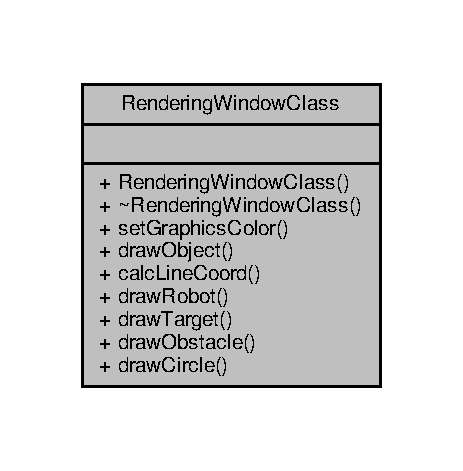
\includegraphics[width=222pt]{classRenderingWindowClass__coll__graph}
\end{center}
\end{figure}
\subsection*{Public Member Functions}
\begin{DoxyCompactItemize}
\item 
\hyperlink{classRenderingWindowClass_ad48948a08088e973aac8a57c96dee52c}{Rendering\-Window\-Class} ()
\begin{DoxyCompactList}\small\item\em Default constructor for \hyperlink{classRenderingWindowClass}{Rendering\-Window\-Class}. \end{DoxyCompactList}\item 
\hypertarget{classRenderingWindowClass_a10c28c3d432aa2e7864284301496fa85}{\hyperlink{classRenderingWindowClass_a10c28c3d432aa2e7864284301496fa85}{$\sim$\-Rendering\-Window\-Class} ()}\label{classRenderingWindowClass_a10c28c3d432aa2e7864284301496fa85}

\begin{DoxyCompactList}\small\item\em Default destructor for \hyperlink{classRenderingWindowClass}{Rendering\-Window\-Class}. \end{DoxyCompactList}\item 
int $\ast$ \hyperlink{classRenderingWindowClass_a57edbe70d96c699103a4f4e2d34736d5}{set\-Graphics\-Color} (\hyperlink{classPhysicalObjectClass}{Physical\-Object\-Class} $\ast$object)
\begin{DoxyCompactList}\small\item\em Populates an array of obstacles/targets to be drawn in the simulation. \end{DoxyCompactList}\item 
void \hyperlink{classRenderingWindowClass_a633f976d7c799676075d3f8025c00006}{draw\-Object} (\hyperlink{classPhysicalObjectClass}{Physical\-Object\-Class} $\ast$object)
\begin{DoxyCompactList}\small\item\em Determines how to draw a \hyperlink{classPhysicalObjectClass}{Physical\-Object\-Class} object. \end{DoxyCompactList}\item 
double $\ast$ \hyperlink{classRenderingWindowClass_af2f7cb3cba6db0f30515d6b66025ca2a}{calc\-Line\-Coord} (double robot\-\_\-\-X, double robot\-\_\-\-Y, double size, double orient)
\begin{DoxyCompactList}\small\item\em Calculates the outside coordinate of the robot's orientation line. \end{DoxyCompactList}\item 
void \hyperlink{classRenderingWindowClass_a1df618c6a1ceddc801b30d6cd15171e9}{draw\-Robot} (\hyperlink{classRobotClass}{Robot\-Class} $\ast$robot)
\begin{DoxyCompactList}\small\item\em Draws the robot with its orientation line. \end{DoxyCompactList}\item 
void \hyperlink{classRenderingWindowClass_a27fe156f6e76032ee94dff6278e76aa8}{draw\-Target} (\hyperlink{classTargetClass}{Target\-Class} $\ast$target)
\begin{DoxyCompactList}\small\item\em Draws a \hyperlink{classTargetClass}{Target\-Class} target. \end{DoxyCompactList}\item 
void \hyperlink{classRenderingWindowClass_a3417e29ad319c3dce14015fc6654fd37}{draw\-Obstacle} (\hyperlink{classObstacleClass}{Obstacle\-Class} $\ast$obstacle)
\begin{DoxyCompactList}\small\item\em Draws an \hyperlink{classObstacleClass}{Obstacle\-Class} obstacle. \end{DoxyCompactList}\item 
\hypertarget{classRenderingWindowClass_a0e97b741d5bac11cef3d09e01543a252}{void {\bfseries draw\-Circle} (double object\-\_\-\-X, double object\-\_\-\-Y, double object\-\_\-size, \hyperlink{classPhysicalObjectClass}{Physical\-Object\-Class} $\ast$object)}\label{classRenderingWindowClass_a0e97b741d5bac11cef3d09e01543a252}

\end{DoxyCompactItemize}


\subsection{Constructor \& Destructor Documentation}
\hypertarget{classRenderingWindowClass_ad48948a08088e973aac8a57c96dee52c}{\index{Rendering\-Window\-Class@{Rendering\-Window\-Class}!Rendering\-Window\-Class@{Rendering\-Window\-Class}}
\index{Rendering\-Window\-Class@{Rendering\-Window\-Class}!RenderingWindowClass@{Rendering\-Window\-Class}}
\subsubsection[{Rendering\-Window\-Class}]{\setlength{\rightskip}{0pt plus 5cm}Rendering\-Window\-Class\-::\-Rendering\-Window\-Class (
\begin{DoxyParamCaption}
{}
\end{DoxyParamCaption}
)}}\label{classRenderingWindowClass_ad48948a08088e973aac8a57c96dee52c}


Default constructor for \hyperlink{classRenderingWindowClass}{Rendering\-Window\-Class}. 

This constructor takes in no arguments. 

\subsection{Member Function Documentation}
\hypertarget{classRenderingWindowClass_af2f7cb3cba6db0f30515d6b66025ca2a}{\index{Rendering\-Window\-Class@{Rendering\-Window\-Class}!calc\-Line\-Coord@{calc\-Line\-Coord}}
\index{calc\-Line\-Coord@{calc\-Line\-Coord}!RenderingWindowClass@{Rendering\-Window\-Class}}
\subsubsection[{calc\-Line\-Coord}]{\setlength{\rightskip}{0pt plus 5cm}double $\ast$ Rendering\-Window\-Class\-::calc\-Line\-Coord (
\begin{DoxyParamCaption}
\item[{double}]{robot\-\_\-\-X, }
\item[{double}]{robot\-\_\-\-Y, }
\item[{double}]{size, }
\item[{double}]{orient}
\end{DoxyParamCaption}
)}}\label{classRenderingWindowClass_af2f7cb3cba6db0f30515d6b66025ca2a}


Calculates the outside coordinate of the robot's orientation line. 

calc\-Line\-Coord takes in the robot's location (robot\-\_\-\-X, robot\-\_\-\-Y), size, and orientation as arguments. The robot's orientation line is anchored to its center at the coordinate (robot\-\_\-\-X, robot\-\_\-\-Y). This method calculates the coordinate of the other end of the line, emerging from the robot (by 20 pixels), based on the robot's orientation. It returns the pointer to an array containing these coordinates so that they can be passed to draw\-Robot.


\begin{DoxyParams}{Parameters}
{\em robot\-\_\-\-X} & double x-\/coordinate of the robot (in pixels) \\
\hline
{\em robot\-\_\-\-Y} & double y-\/coordinate of the robot (in pixels) \\
\hline
{\em size} & double size of the robot (in pixels) \\
\hline
{\em orient} & double orientation of the robot (in degrees; 0 as the positive x-\/axis) \\
\hline
\end{DoxyParams}
\begin{DoxyReturn}{Returns}
calc\-Line\-Coord pointer to double array containing end coordinates of orientation line 
\end{DoxyReturn}
\hypertarget{classRenderingWindowClass_a633f976d7c799676075d3f8025c00006}{\index{Rendering\-Window\-Class@{Rendering\-Window\-Class}!draw\-Object@{draw\-Object}}
\index{draw\-Object@{draw\-Object}!RenderingWindowClass@{Rendering\-Window\-Class}}
\subsubsection[{draw\-Object}]{\setlength{\rightskip}{0pt plus 5cm}void Rendering\-Window\-Class\-::draw\-Object (
\begin{DoxyParamCaption}
\item[{{\bf Physical\-Object\-Class} $\ast$}]{object}
\end{DoxyParamCaption}
)}}\label{classRenderingWindowClass_a633f976d7c799676075d3f8025c00006}


Determines how to draw a \hyperlink{classPhysicalObjectClass}{Physical\-Object\-Class} object. 

draw\-Object takes in a \hyperlink{classPhysicalObjectClass}{Physical\-Object\-Class} object as an argument and decides based on the object's Object\-Type attribute (robot, target, or obstacle) whether to draw the object as a robot, target, or obstacle, respectively. If an invalid Object\-Type is detected, the object is not drawn.


\begin{DoxyParams}{Parameters}
{\em object} & a \hyperlink{classPhysicalObjectClass}{Physical\-Object\-Class} object within the simulation \\
\hline
\end{DoxyParams}
\hypertarget{classRenderingWindowClass_a3417e29ad319c3dce14015fc6654fd37}{\index{Rendering\-Window\-Class@{Rendering\-Window\-Class}!draw\-Obstacle@{draw\-Obstacle}}
\index{draw\-Obstacle@{draw\-Obstacle}!RenderingWindowClass@{Rendering\-Window\-Class}}
\subsubsection[{draw\-Obstacle}]{\setlength{\rightskip}{0pt plus 5cm}void Rendering\-Window\-Class\-::draw\-Obstacle (
\begin{DoxyParamCaption}
\item[{{\bf Obstacle\-Class} $\ast$}]{obstacle}
\end{DoxyParamCaption}
)}}\label{classRenderingWindowClass_a3417e29ad319c3dce14015fc6654fd37}


Draws an \hyperlink{classObstacleClass}{Obstacle\-Class} obstacle. 

draw\-Obstacle takes in a \hyperlink{classObstacleClass}{Obstacle\-Class} obstacle object as an argument. For Iteration 2, it draws the obstacle as a circle of radius \char`\"{}size\char`\"{} using 50 triangle fans. The color of the obstacle is determined by the object's color attribute.


\begin{DoxyParams}{Parameters}
{\em obstacle} & an obstacle within the simulation \\
\hline
\end{DoxyParams}
\hypertarget{classRenderingWindowClass_a1df618c6a1ceddc801b30d6cd15171e9}{\index{Rendering\-Window\-Class@{Rendering\-Window\-Class}!draw\-Robot@{draw\-Robot}}
\index{draw\-Robot@{draw\-Robot}!RenderingWindowClass@{Rendering\-Window\-Class}}
\subsubsection[{draw\-Robot}]{\setlength{\rightskip}{0pt plus 5cm}void Rendering\-Window\-Class\-::draw\-Robot (
\begin{DoxyParamCaption}
\item[{{\bf Robot\-Class} $\ast$}]{robot}
\end{DoxyParamCaption}
)}}\label{classRenderingWindowClass_a1df618c6a1ceddc801b30d6cd15171e9}


Draws the robot with its orientation line. 

draw\-Robot takes in a \hyperlink{classRobotClass}{Robot\-Class} robot object as an argument. It draws the main body of the robot as a circle of radius \char`\"{}size\char`\"{} using 50 triangle fans. Then it draws a line anchored at the center of the robot and emerging from its body in the direction of its orientation. The default robot body color is green, and the default orientation line color is red.


\begin{DoxyParams}{Parameters}
{\em robot} & a robot within the simulation \\
\hline
\end{DoxyParams}
\hypertarget{classRenderingWindowClass_a27fe156f6e76032ee94dff6278e76aa8}{\index{Rendering\-Window\-Class@{Rendering\-Window\-Class}!draw\-Target@{draw\-Target}}
\index{draw\-Target@{draw\-Target}!RenderingWindowClass@{Rendering\-Window\-Class}}
\subsubsection[{draw\-Target}]{\setlength{\rightskip}{0pt plus 5cm}void Rendering\-Window\-Class\-::draw\-Target (
\begin{DoxyParamCaption}
\item[{{\bf Target\-Class} $\ast$}]{target}
\end{DoxyParamCaption}
)}}\label{classRenderingWindowClass_a27fe156f6e76032ee94dff6278e76aa8}


Draws a \hyperlink{classTargetClass}{Target\-Class} target. 

draw\-Target takes in a \hyperlink{classTargetClass}{Target\-Class} target object as an argument. For Iteration 2, it draws the target as a circle of radius \char`\"{}size\char`\"{} using 50 triangle fans. The color of the target is determined by the object's color attribute.


\begin{DoxyParams}{Parameters}
{\em target} & a target within the simulation \\
\hline
\end{DoxyParams}
\hypertarget{classRenderingWindowClass_a57edbe70d96c699103a4f4e2d34736d5}{\index{Rendering\-Window\-Class@{Rendering\-Window\-Class}!set\-Graphics\-Color@{set\-Graphics\-Color}}
\index{set\-Graphics\-Color@{set\-Graphics\-Color}!RenderingWindowClass@{Rendering\-Window\-Class}}
\subsubsection[{set\-Graphics\-Color}]{\setlength{\rightskip}{0pt plus 5cm}int $\ast$ Rendering\-Window\-Class\-::set\-Graphics\-Color (
\begin{DoxyParamCaption}
\item[{{\bf Physical\-Object\-Class} $\ast$}]{object}
\end{DoxyParamCaption}
)}}\label{classRenderingWindowClass_a57edbe70d96c699103a4f4e2d34736d5}


Populates an array of obstacles/targets to be drawn in the simulation. 

init\-Object takes in one \hyperlink{classObstacleClass}{Obstacle\-Class} type object (an obstacle or a target) as an argument and adds its properties (shape, size, location) to the obstacle\-Array. \hyperlink{Simulation_8cpp}{Simulation.\-cpp} accesses these properties through the obstacle\-Array when displaying the objects in the G\-L\-U\-T window. At the beginning of the simulation, the variable int num\-Of\-Objects is set to 0. After an object is added to the obstacle\-Array, this counter is incremented so that the next object will be added to the next slot in the array.


\begin{DoxyParams}{Parameters}
{\em object} & a robot/target/obstacle added to the environment's physical\-Object\-Vector\-Determines how to render the color a \hyperlink{classPhysicalObjectClass}{Physical\-Object\-Class} object\\
\hline
\end{DoxyParams}
set\-Graphics\-Color takes in a \hyperlink{classPhysicalObjectClass}{Physical\-Object\-Class} object as an argument and decides based on the object's color attribute which parameters to pass to G\-L\-U\-T's gl\-Color3f function, which is called in the draw\-Circle method (and any future methods for drawing different shapes).


\begin{DoxyParams}{Parameters}
{\em object} & a \hyperlink{classPhysicalObjectClass}{Physical\-Object\-Class} object within the simulation \\
\hline
\end{DoxyParams}


The documentation for this class was generated from the following files\-:\begin{DoxyCompactItemize}
\item 
\hyperlink{RenderingWindowClass_8h}{Rendering\-Window\-Class.\-h}\item 
\hyperlink{RenderingWindowClass_8cpp}{Rendering\-Window\-Class.\-cpp}\end{DoxyCompactItemize}

\hypertarget{classRobotClass}{\section{Robot\-Class Class Reference}
\label{classRobotClass}\index{Robot\-Class@{Robot\-Class}}
}


Inheritance diagram for Robot\-Class\-:
\nopagebreak
\begin{figure}[H]
\begin{center}
\leavevmode
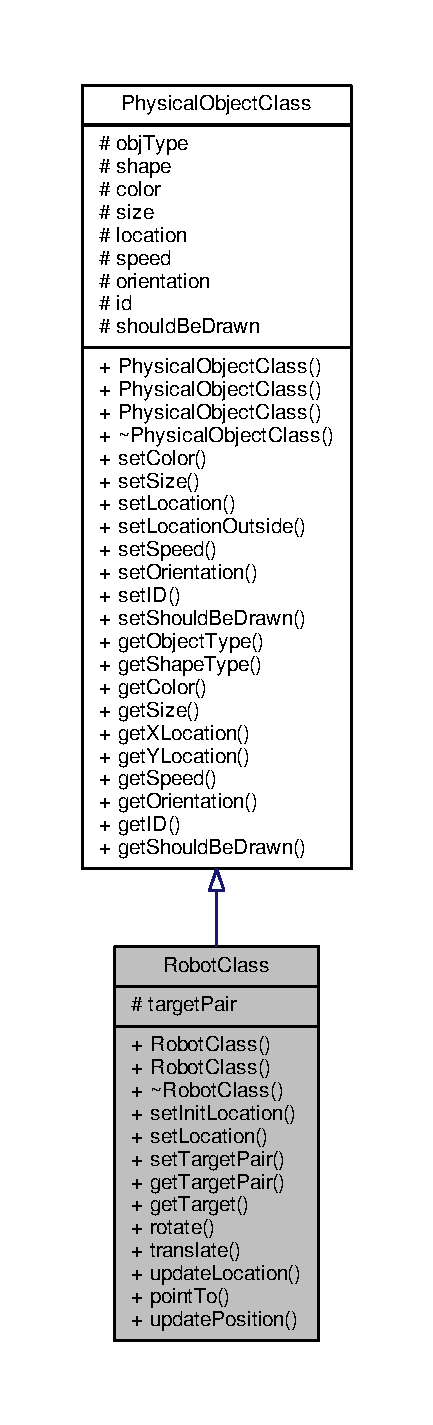
\includegraphics[height=550pt]{classRobotClass__inherit__graph}
\end{center}
\end{figure}


Collaboration diagram for Robot\-Class\-:
\nopagebreak
\begin{figure}[H]
\begin{center}
\leavevmode
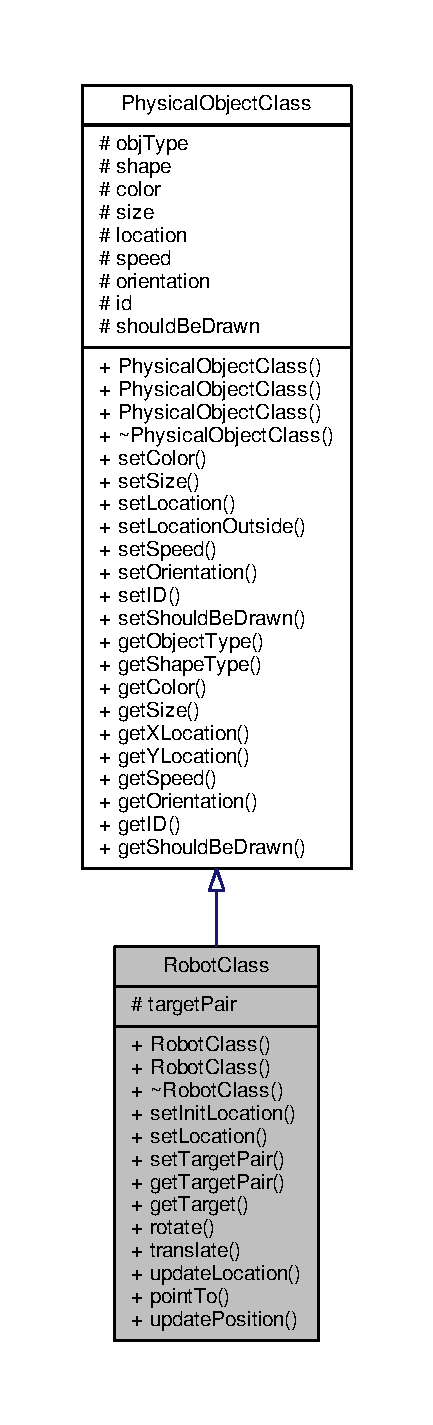
\includegraphics[height=550pt]{classRobotClass__coll__graph}
\end{center}
\end{figure}
\subsection*{Public Member Functions}
\begin{DoxyCompactItemize}
\item 
\hyperlink{classRobotClass_a7125604039c2a4b39e34e4354bd4ce19}{Robot\-Class} ()
\begin{DoxyCompactList}\small\item\em Default constructor for \hyperlink{classRobotClass}{Robot\-Class}. \end{DoxyCompactList}\item 
\hyperlink{classRobotClass_a5fc34d4751e7af1868eefec70ecbe241}{Robot\-Class} (int size\-In, double x, double y)
\begin{DoxyCompactList}\small\item\em Constructor with three arguments, size\-In, x, and y. \end{DoxyCompactList}\item 
\hypertarget{classRobotClass_a7d7725737f146f85ed7ceeae7f300e9e}{\hyperlink{classRobotClass_a7d7725737f146f85ed7ceeae7f300e9e}{$\sim$\-Robot\-Class} ()}\label{classRobotClass_a7d7725737f146f85ed7ceeae7f300e9e}

\begin{DoxyCompactList}\small\item\em default deconstructor for \hyperlink{classRobotClass}{Robot\-Class} \end{DoxyCompactList}\item 
void \hyperlink{classRobotClass_a6e4902a26041b33ed83932a4514bb8c0}{set\-Init\-Location} (double x, double y)
\begin{DoxyCompactList}\small\item\em Sets the initial robot location. \end{DoxyCompactList}\item 
\hypertarget{classRobotClass_a264d12c67f65e3eef63a0e90a3b902b1}{void \hyperlink{classRobotClass_a264d12c67f65e3eef63a0e90a3b902b1}{set\-Location} (double x, double y)}\label{classRobotClass_a264d12c67f65e3eef63a0e90a3b902b1}

\begin{DoxyCompactList}\small\item\em Sets the robot location. \end{DoxyCompactList}\item 
void \hyperlink{classRobotClass_a846281a36ffd93349b2d9df7ef009ba5}{set\-Target\-Pair} (int target)
\begin{DoxyCompactList}\small\item\em Associates target with robot. \end{DoxyCompactList}\item 
int \hyperlink{classRobotClass_a6917e8e0466c4fe0e6827d2c1542c012}{get\-Target\-Pair} ()
\begin{DoxyCompactList}\small\item\em Returns the unique signal of the target to which the robot is paired. \end{DoxyCompactList}\item 
\hyperlink{classPhysicalObjectClass}{Physical\-Object\-Class} $\ast$ \hyperlink{classRobotClass_a12c66f3be1dd345448398e811ebc5787}{get\-Target} ()
\begin{DoxyCompactList}\small\item\em Returns the target to which the robot is paired. \end{DoxyCompactList}\item 
void \hyperlink{classRobotClass_af0a67d59620139069f981da208a7a28d}{rotate} (int degrees)
\begin{DoxyCompactList}\small\item\em rotates the robot while moving \end{DoxyCompactList}\item 
\hypertarget{classRobotClass_aea48d75ac942eef8e7d0891784f48e0b}{void \hyperlink{classRobotClass_aea48d75ac942eef8e7d0891784f48e0b}{translate} (int pixels)}\label{classRobotClass_aea48d75ac942eef8e7d0891784f48e0b}

\begin{DoxyCompactList}\small\item\em moves the robot \end{DoxyCompactList}\item 
\hypertarget{classRobotClass_a1ce57ed179b9816eb492613bcfd65afb}{void \hyperlink{classRobotClass_a1ce57ed179b9816eb492613bcfd65afb}{update\-Location} ()}\label{classRobotClass_a1ce57ed179b9816eb492613bcfd65afb}

\begin{DoxyCompactList}\small\item\em updates robot's position \end{DoxyCompactList}\item 
\hypertarget{classRobotClass_a5de1615cb1128b98a87cbba7933c11c6}{void \hyperlink{classRobotClass_a5de1615cb1128b98a87cbba7933c11c6}{point\-To} ()}\label{classRobotClass_a5de1615cb1128b98a87cbba7933c11c6}

\begin{DoxyCompactList}\small\item\em sets the orientation of robot to target \end{DoxyCompactList}\item 
\hypertarget{classRobotClass_a0d57b2a1df5b361d5117f3deb2e3eb4e}{void {\bfseries update\-Position} ()}\label{classRobotClass_a0d57b2a1df5b361d5117f3deb2e3eb4e}

\end{DoxyCompactItemize}
\subsection*{Protected Attributes}
\begin{DoxyCompactItemize}
\item 
\hypertarget{classRobotClass_a6b3abefce8010c6e3b31a7d8546fe3fb}{int {\bfseries target\-Pair}}\label{classRobotClass_a6b3abefce8010c6e3b31a7d8546fe3fb}

\end{DoxyCompactItemize}


\subsection{Constructor \& Destructor Documentation}
\hypertarget{classRobotClass_a7125604039c2a4b39e34e4354bd4ce19}{\index{Robot\-Class@{Robot\-Class}!Robot\-Class@{Robot\-Class}}
\index{Robot\-Class@{Robot\-Class}!RobotClass@{Robot\-Class}}
\subsubsection[{Robot\-Class}]{\setlength{\rightskip}{0pt plus 5cm}Robot\-Class\-::\-Robot\-Class (
\begin{DoxyParamCaption}
{}
\end{DoxyParamCaption}
)}}\label{classRobotClass_a7125604039c2a4b39e34e4354bd4ce19}


Default constructor for \hyperlink{classRobotClass}{Robot\-Class}. 

This constructor takes in no arguments and sets the circle to a random location with size 50 and speed 10 \hypertarget{classRobotClass_a5fc34d4751e7af1868eefec70ecbe241}{\index{Robot\-Class@{Robot\-Class}!Robot\-Class@{Robot\-Class}}
\index{Robot\-Class@{Robot\-Class}!RobotClass@{Robot\-Class}}
\subsubsection[{Robot\-Class}]{\setlength{\rightskip}{0pt plus 5cm}Robot\-Class\-::\-Robot\-Class (
\begin{DoxyParamCaption}
\item[{int}]{size\-In, }
\item[{double}]{x, }
\item[{double}]{y}
\end{DoxyParamCaption}
)}}\label{classRobotClass_a5fc34d4751e7af1868eefec70ecbe241}


Constructor with three arguments, size\-In, x, and y. 

This constructor takes in three integer arguments. The first, size\-In, determines the size of the robot. The other arguments, x and y, determine its location


\begin{DoxyParams}{Parameters}
{\em size\-In} & integer size of the robot \\
\hline
{\em x} & x double location of the robot \\
\hline
{\em y} & y double location of the robot \\
\hline
\end{DoxyParams}


\subsection{Member Function Documentation}
\hypertarget{classRobotClass_a12c66f3be1dd345448398e811ebc5787}{\index{Robot\-Class@{Robot\-Class}!get\-Target@{get\-Target}}
\index{get\-Target@{get\-Target}!RobotClass@{Robot\-Class}}
\subsubsection[{get\-Target}]{\setlength{\rightskip}{0pt plus 5cm}{\bf Physical\-Object\-Class} $\ast$ Robot\-Class\-::get\-Target (
\begin{DoxyParamCaption}
{}
\end{DoxyParamCaption}
)}}\label{classRobotClass_a12c66f3be1dd345448398e811ebc5787}


Returns the target to which the robot is paired. 

\begin{DoxyReturn}{Returns}
\hyperlink{classTargetClass}{Target\-Class} target 
\end{DoxyReturn}
\hypertarget{classRobotClass_a6917e8e0466c4fe0e6827d2c1542c012}{\index{Robot\-Class@{Robot\-Class}!get\-Target\-Pair@{get\-Target\-Pair}}
\index{get\-Target\-Pair@{get\-Target\-Pair}!RobotClass@{Robot\-Class}}
\subsubsection[{get\-Target\-Pair}]{\setlength{\rightskip}{0pt plus 5cm}int Robot\-Class\-::get\-Target\-Pair (
\begin{DoxyParamCaption}
{}
\end{DoxyParamCaption}
)}}\label{classRobotClass_a6917e8e0466c4fe0e6827d2c1542c012}


Returns the unique signal of the target to which the robot is paired. 

\begin{DoxyReturn}{Returns}
integer target\-Pair 
\end{DoxyReturn}
\hypertarget{classRobotClass_af0a67d59620139069f981da208a7a28d}{\index{Robot\-Class@{Robot\-Class}!rotate@{rotate}}
\index{rotate@{rotate}!RobotClass@{Robot\-Class}}
\subsubsection[{rotate}]{\setlength{\rightskip}{0pt plus 5cm}void Robot\-Class\-::rotate (
\begin{DoxyParamCaption}
\item[{int}]{degrees}
\end{DoxyParamCaption}
)}}\label{classRobotClass_af0a67d59620139069f981da208a7a28d}


rotates the robot while moving 

\begin{DoxyReturn}{Returns}
true if there's a wall

true if a particular obstacle is close

true if there is an obstacle
\end{DoxyReturn}
This function takes in an integer argument, degrees, and rotates the object the amount specified. Positive rotates counter clockwise, the opposite for negative.


\begin{DoxyParams}{Parameters}
{\em degrees} & integer argument specifying rotation amount \\
\hline
\end{DoxyParams}
\hypertarget{classRobotClass_a6e4902a26041b33ed83932a4514bb8c0}{\index{Robot\-Class@{Robot\-Class}!set\-Init\-Location@{set\-Init\-Location}}
\index{set\-Init\-Location@{set\-Init\-Location}!RobotClass@{Robot\-Class}}
\subsubsection[{set\-Init\-Location}]{\setlength{\rightskip}{0pt plus 5cm}void Robot\-Class\-::set\-Init\-Location (
\begin{DoxyParamCaption}
\item[{double}]{x, }
\item[{double}]{y}
\end{DoxyParamCaption}
)}}\label{classRobotClass_a6e4902a26041b33ed83932a4514bb8c0}


Sets the initial robot location. 

Sets the initial robot location, ensuring that the robot will not overlap with any other objects


\begin{DoxyParams}{Parameters}
{\em x} & x double location of the robot \\
\hline
{\em y} & y double location of the robot \\
\hline
\end{DoxyParams}
\hypertarget{classRobotClass_a846281a36ffd93349b2d9df7ef009ba5}{\index{Robot\-Class@{Robot\-Class}!set\-Target\-Pair@{set\-Target\-Pair}}
\index{set\-Target\-Pair@{set\-Target\-Pair}!RobotClass@{Robot\-Class}}
\subsubsection[{set\-Target\-Pair}]{\setlength{\rightskip}{0pt plus 5cm}void Robot\-Class\-::set\-Target\-Pair (
\begin{DoxyParamCaption}
\item[{int}]{target}
\end{DoxyParamCaption}
)}}\label{classRobotClass_a846281a36ffd93349b2d9df7ef009ba5}


Associates target with robot. 


\begin{DoxyParams}{Parameters}
{\em target} & integer representation of a target \\
\hline
\end{DoxyParams}


The documentation for this class was generated from the following files\-:\begin{DoxyCompactItemize}
\item 
\hyperlink{RobotClass_8h}{Robot\-Class.\-h}\item 
\hyperlink{RobotClass_8cpp}{Robot\-Class.\-cpp}\end{DoxyCompactItemize}

\hypertarget{classSimulation}{\section{Simulation Class Reference}
\label{classSimulation}\index{Simulation@{Simulation}}
}


{\ttfamily \#include $<$Simulation.\-h$>$}



Inheritance diagram for Simulation\-:\nopagebreak
\begin{figure}[H]
\begin{center}
\leavevmode
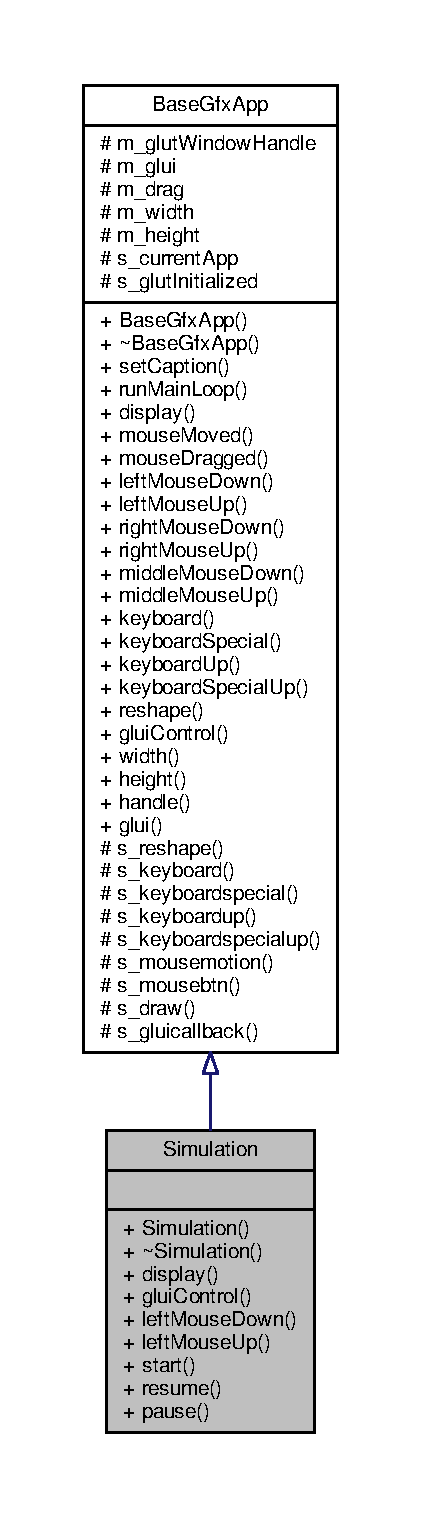
\includegraphics[height=550pt]{classSimulation__inherit__graph}
\end{center}
\end{figure}


Collaboration diagram for Simulation\-:\nopagebreak
\begin{figure}[H]
\begin{center}
\leavevmode
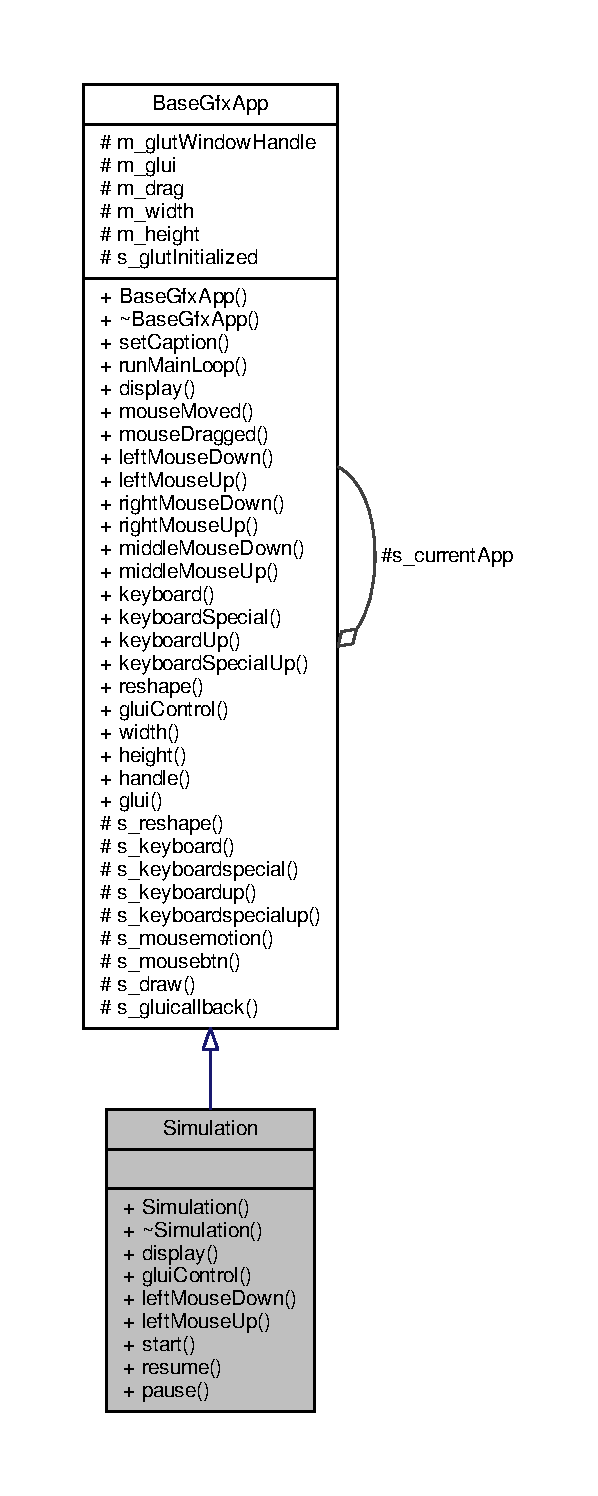
\includegraphics[height=550pt]{classSimulation__coll__graph}
\end{center}
\end{figure}
\subsection*{Public Types}
\begin{DoxyCompactItemize}
\item 
enum {\bfseries U\-I\-Control\-Type} \{ {\bfseries U\-I\-\_\-\-Q\-U\-I\-T} = 0
 \}
\end{DoxyCompactItemize}
\subsection*{Public Member Functions}
\begin{DoxyCompactItemize}
\item 
\hyperlink{classSimulation_a4c669ceaa34c7130966ce45f9de75fbe}{Simulation} (int argc, char $\ast$argv\mbox{[}$\,$\mbox{]}, int width, int height)
\begin{DoxyCompactList}\small\item\em Initializes Open\-G\-L window. \end{DoxyCompactList}\item 
void \hyperlink{classSimulation_a449dcb7d97dfba99efe770de2f399c31}{display} ()
\begin{DoxyCompactList}\small\item\em Displays objects. \end{DoxyCompactList}\item 
\hypertarget{classSimulation_a1607cd18e552ab9f4a6f57d362f7121a}{void {\bfseries glui\-Control} (int control\-I\-D)}\label{classSimulation_a1607cd18e552ab9f4a6f57d362f7121a}

\item 
\hypertarget{classSimulation_a786d1ba31d29937f0ac6f3ea88f8a607}{void {\bfseries left\-Mouse\-Down} (int x, int y)}\label{classSimulation_a786d1ba31d29937f0ac6f3ea88f8a607}

\item 
\hypertarget{classSimulation_a62ef254d85017074cd521a5787b5a234}{void {\bfseries left\-Mouse\-Up} (int x, int y)}\label{classSimulation_a62ef254d85017074cd521a5787b5a234}

\end{DoxyCompactItemize}
\subsection*{Static Public Member Functions}
\begin{DoxyCompactItemize}
\item 
static void \hyperlink{classSimulation_acfbe29877511e1db19de6228c0f0caa2}{start} (int id)
\begin{DoxyCompactList}\small\item\em Starts simulation. \end{DoxyCompactList}\item 
static void \hyperlink{classSimulation_a8d1e79b53836e7f99d1946b9148c2400}{resume} (int id)
\begin{DoxyCompactList}\small\item\em Resumes simulation. \end{DoxyCompactList}\item 
static void \hyperlink{classSimulation_a8c8072e3d10589704d12aa3f3d8ef1e0}{pause} (int id)
\begin{DoxyCompactList}\small\item\em Pauses simulation. \end{DoxyCompactList}\end{DoxyCompactItemize}
\subsection*{Additional Inherited Members}


\subsection{Detailed Description}
The \hyperlink{classSimulation}{Simulation} class. This sets up the G\-U\-I and the drawing environment. 

\subsection{Constructor \& Destructor Documentation}
\hypertarget{classSimulation_a4c669ceaa34c7130966ce45f9de75fbe}{\index{Simulation@{Simulation}!Simulation@{Simulation}}
\index{Simulation@{Simulation}!Simulation@{Simulation}}
\subsubsection[{Simulation}]{\setlength{\rightskip}{0pt plus 5cm}Simulation\-::\-Simulation (
\begin{DoxyParamCaption}
\item[{int}]{argc, }
\item[{char $\ast$}]{argv\mbox{[}$\,$\mbox{]}, }
\item[{int}]{width, }
\item[{int}]{height}
\end{DoxyParamCaption}
)}}\label{classSimulation_a4c669ceaa34c7130966ce45f9de75fbe}


Initializes Open\-G\-L window. 

Creates Open\-G\-L window and basic U\-I panel with quit button. 

\subsection{Member Function Documentation}
\hypertarget{classSimulation_a449dcb7d97dfba99efe770de2f399c31}{\index{Simulation@{Simulation}!display@{display}}
\index{display@{display}!Simulation@{Simulation}}
\subsubsection[{display}]{\setlength{\rightskip}{0pt plus 5cm}void Simulation\-::display (
\begin{DoxyParamCaption}
{}
\end{DoxyParamCaption}
)\hspace{0.3cm}{\ttfamily [virtual]}}}\label{classSimulation_a449dcb7d97dfba99efe770de2f399c31}


Displays objects. 

This function takes objects from obstacle\-Array and displays them in the Open\-G\-L window by calling the drawing functions from drawing.\-cpp. The function then checks to make sure that the robot does not overlap the obstacles or target. The location of the robot is reset with random coordinates until it doesn't overlap any obstacles or the target. Then draws and displays robot. 

Reimplemented from \hyperlink{classBaseGfxApp}{Base\-Gfx\-App}.

\hypertarget{classSimulation_a8c8072e3d10589704d12aa3f3d8ef1e0}{\index{Simulation@{Simulation}!pause@{pause}}
\index{pause@{pause}!Simulation@{Simulation}}
\subsubsection[{pause}]{\setlength{\rightskip}{0pt plus 5cm}void Simulation\-::pause (
\begin{DoxyParamCaption}
\item[{int}]{id}
\end{DoxyParamCaption}
)\hspace{0.3cm}{\ttfamily [static]}}}\label{classSimulation_a8c8072e3d10589704d12aa3f3d8ef1e0}


Pauses simulation. 

Pauses simulation by toggling flag. This prevents the environment from running the update function by returning at the beginning. This prevents objects from updating any attributes, effectively \char`\"{}pausing\char`\"{} the simulation.


\begin{DoxyParams}{Parameters}
{\em id} & button identifier to be used in future iterations \\
\hline
\end{DoxyParams}
\hypertarget{classSimulation_a8d1e79b53836e7f99d1946b9148c2400}{\index{Simulation@{Simulation}!resume@{resume}}
\index{resume@{resume}!Simulation@{Simulation}}
\subsubsection[{resume}]{\setlength{\rightskip}{0pt plus 5cm}void Simulation\-::resume (
\begin{DoxyParamCaption}
\item[{int}]{id}
\end{DoxyParamCaption}
)\hspace{0.3cm}{\ttfamily [static]}}}\label{classSimulation_a8d1e79b53836e7f99d1946b9148c2400}


Resumes simulation. 

Resumes simulation after pausing by toggling flag. This allows the environment to resume running the update function.


\begin{DoxyParams}{Parameters}
{\em id} & button identifier to be used in future iterations \\
\hline
\end{DoxyParams}
\hypertarget{classSimulation_acfbe29877511e1db19de6228c0f0caa2}{\index{Simulation@{Simulation}!start@{start}}
\index{start@{start}!Simulation@{Simulation}}
\subsubsection[{start}]{\setlength{\rightskip}{0pt plus 5cm}void Simulation\-::start (
\begin{DoxyParamCaption}
\item[{int}]{id}
\end{DoxyParamCaption}
)\hspace{0.3cm}{\ttfamily [static]}}}\label{classSimulation_acfbe29877511e1db19de6228c0f0caa2}


Starts simulation. 

Starts simulation by toggling flag. This allows the environment to run the update function and move the objects.


\begin{DoxyParams}{Parameters}
{\em id} & button identifier to be used in future iterations \\
\hline
\end{DoxyParams}


The documentation for this class was generated from the following files\-:\begin{DoxyCompactItemize}
\item 
\hyperlink{Simulation_8h}{Simulation.\-h}\item 
\hyperlink{Simulation_8cpp}{Simulation.\-cpp}\end{DoxyCompactItemize}

\hypertarget{classTargetClass}{\section{Target\-Class Class Reference}
\label{classTargetClass}\index{Target\-Class@{Target\-Class}}
}


Inheritance diagram for Target\-Class\-:
\nopagebreak
\begin{figure}[H]
\begin{center}
\leavevmode
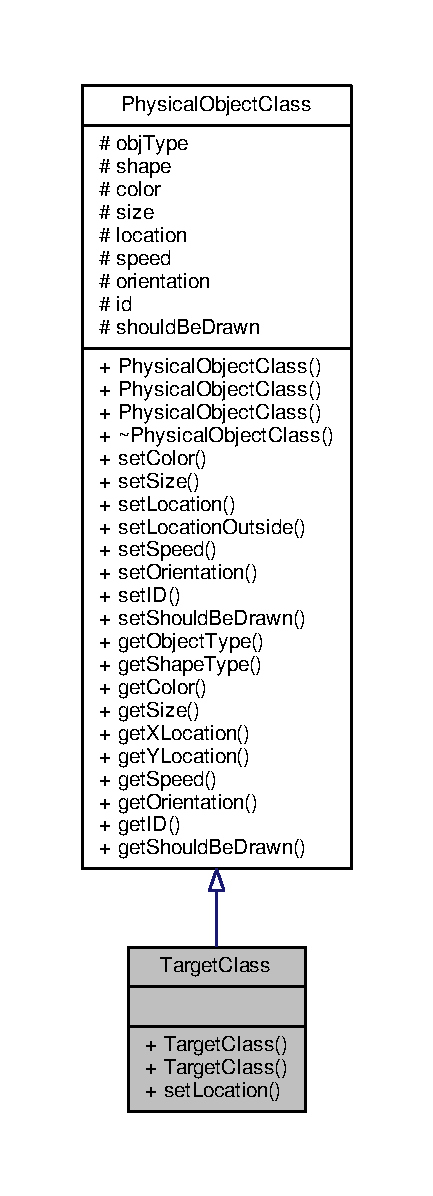
\includegraphics[height=550pt]{classTargetClass__inherit__graph}
\end{center}
\end{figure}


Collaboration diagram for Target\-Class\-:
\nopagebreak
\begin{figure}[H]
\begin{center}
\leavevmode
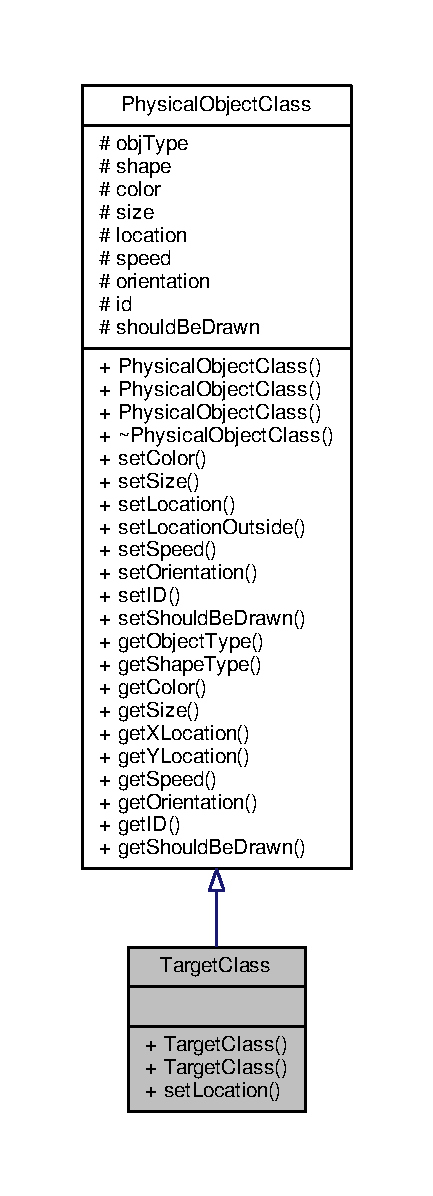
\includegraphics[height=550pt]{classTargetClass__coll__graph}
\end{center}
\end{figure}
\subsection*{Public Member Functions}
\begin{DoxyCompactItemize}
\item 
\hypertarget{classTargetClass_aa851f8197d417b015e21f060442bfc88}{\hyperlink{classTargetClass_aa851f8197d417b015e21f060442bfc88}{Target\-Class} ()}\label{classTargetClass_aa851f8197d417b015e21f060442bfc88}

\begin{DoxyCompactList}\small\item\em default constructor for \hyperlink{classEnvironmentClass}{Environment\-Class} \end{DoxyCompactList}\item 
\hypertarget{classTargetClass_a94f1a6460368b44849aedcc7a4e46fc4}{\hyperlink{classTargetClass_a94f1a6460368b44849aedcc7a4e46fc4}{Target\-Class} (char color\-In)}\label{classTargetClass_a94f1a6460368b44849aedcc7a4e46fc4}

\begin{DoxyCompactList}\small\item\em constructor for \hyperlink{classEnvironmentClass}{Environment\-Class} that takes in color \end{DoxyCompactList}\item 
void \hyperlink{classTargetClass_ac6d882304b638f48e5cab2a1b5b82551}{set\-Location} (double x, double y)
\begin{DoxyCompactList}\small\item\em Set the target location. \end{DoxyCompactList}\end{DoxyCompactItemize}
\subsection*{Additional Inherited Members}


\subsection{Member Function Documentation}
\hypertarget{classTargetClass_ac6d882304b638f48e5cab2a1b5b82551}{\index{Target\-Class@{Target\-Class}!set\-Location@{set\-Location}}
\index{set\-Location@{set\-Location}!TargetClass@{Target\-Class}}
\subsubsection[{set\-Location}]{\setlength{\rightskip}{0pt plus 5cm}void Target\-Class\-::set\-Location (
\begin{DoxyParamCaption}
\item[{double}]{x, }
\item[{double}]{y}
\end{DoxyParamCaption}
)\hspace{0.3cm}{\ttfamily [virtual]}}}\label{classTargetClass_ac6d882304b638f48e5cab2a1b5b82551}


Set the target location. 

This function takes in the double arguments (x, y) and sets its location.


\begin{DoxyParams}{Parameters}
{\em x} & double x-\/coordinate \\
\hline
{\em y} & double y-\/coordinate \\
\hline
\end{DoxyParams}


Reimplemented from \hyperlink{classPhysicalObjectClass_a3f9833aa04aa438de63b82fc761910ba}{Physical\-Object\-Class}.



The documentation for this class was generated from the following files\-:\begin{DoxyCompactItemize}
\item 
\hyperlink{TargetClass_8h}{Target\-Class.\-h}\item 
\hyperlink{TargetClass_8cpp}{Target\-Class.\-cpp}\end{DoxyCompactItemize}

\hypertarget{classTargetClassTests}{\section{Target\-Class\-Tests Class Reference}
\label{classTargetClassTests}\index{Target\-Class\-Tests@{Target\-Class\-Tests}}
}


Inheritance diagram for Target\-Class\-Tests\-:\nopagebreak
\begin{figure}[H]
\begin{center}
\leavevmode
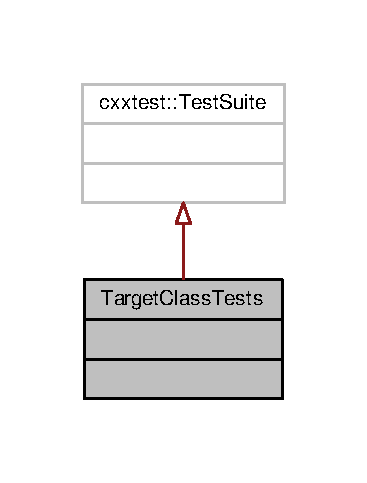
\includegraphics[width=176pt]{classTargetClassTests__inherit__graph}
\end{center}
\end{figure}


Collaboration diagram for Target\-Class\-Tests\-:\nopagebreak
\begin{figure}[H]
\begin{center}
\leavevmode
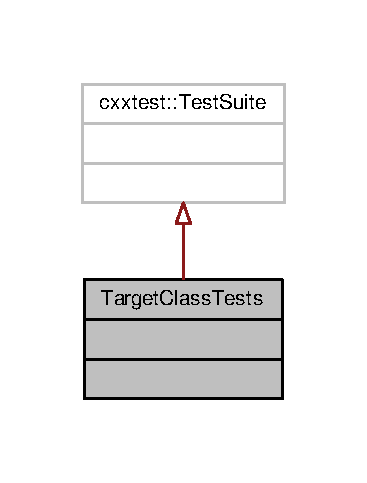
\includegraphics[width=176pt]{classTargetClassTests__coll__graph}
\end{center}
\end{figure}


The documentation for this class was generated from the following file\-:\begin{DoxyCompactItemize}
\item 
Target\-Class\-Tests.\-h\end{DoxyCompactItemize}

\chapter{File Documentation}
\hypertarget{BaseGfxApp_8h}{\section{Base\-Gfx\-App.\-h File Reference}
\label{BaseGfxApp_8h}\index{Base\-Gfx\-App.\-h@{Base\-Gfx\-App.\-h}}
}


The basic application class for C\-Sci-\/3081 project. Uses G\-L\-U\-T and G\-L\-U\-I and wraps them in a nice C++ interface.  


{\ttfamily \#include $<$string$>$}\\*
{\ttfamily \#include $<$iostream$>$}\\*
{\ttfamily \#include $<$assert.\-h$>$}\\*
{\ttfamily \#include $<$G\-L/glui.\-h$>$}\\*
Include dependency graph for Base\-Gfx\-App.\-h\-:\nopagebreak
\begin{figure}[H]
\begin{center}
\leavevmode
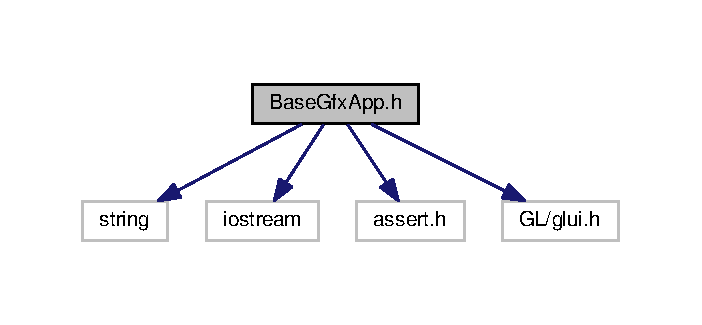
\includegraphics[width=337pt]{BaseGfxApp_8h__incl}
\end{center}
\end{figure}
This graph shows which files directly or indirectly include this file\-:\nopagebreak
\begin{figure}[H]
\begin{center}
\leavevmode
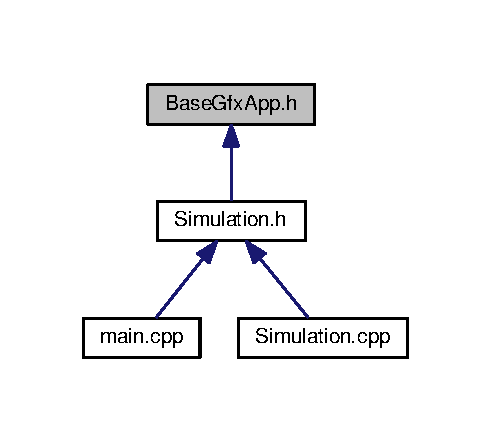
\includegraphics[width=235pt]{BaseGfxApp_8h__dep__incl}
\end{center}
\end{figure}
\subsection*{Classes}
\begin{DoxyCompactItemize}
\item 
class \hyperlink{classBaseGfxApp}{Base\-Gfx\-App}
\end{DoxyCompactItemize}


\subsection{Detailed Description}
The basic application class for C\-Sci-\/3081 project. Uses G\-L\-U\-T and G\-L\-U\-I and wraps them in a nice C++ interface. \begin{DoxyAuthor}{Author}
C\-Sci3081 Guru 
\end{DoxyAuthor}

\input{EnvironmentClass_8cpp}
\input{EnvironmentClass_8h}
\hypertarget{main_8cpp}{\section{main.\-cpp File Reference}
\label{main_8cpp}\index{main.\-cpp@{main.\-cpp}}
}


driver file for robot class  


{\ttfamily \#include \char`\"{}Simulation.\-h\char`\"{}}\\*
{\ttfamily \#include \char`\"{}Environment\-Class.\-h\char`\"{}}\\*
Include dependency graph for main.\-cpp\-:
\nopagebreak
\begin{figure}[H]
\begin{center}
\leavevmode
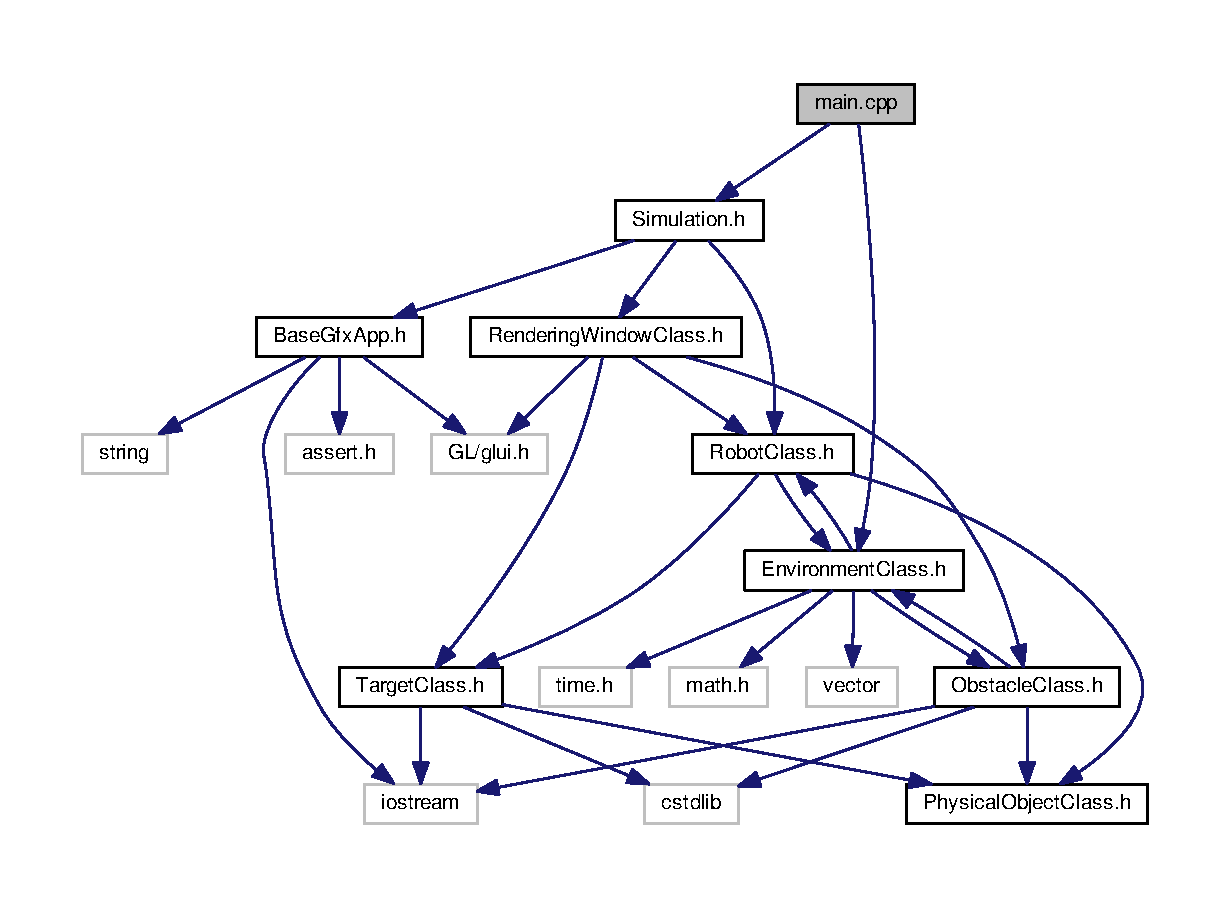
\includegraphics[width=350pt]{main_8cpp__incl}
\end{center}
\end{figure}
\subsection*{Functions}
\begin{DoxyCompactItemize}
\item 
\hypertarget{main_8cpp_a0ddf1224851353fc92bfbff6f499fa97}{int {\bfseries main} (int argc, char $\ast$argv\mbox{[}$\,$\mbox{]})}\label{main_8cpp_a0ddf1224851353fc92bfbff6f499fa97}

\end{DoxyCompactItemize}
\subsection*{Variables}
\begin{DoxyCompactItemize}
\item 
\hypertarget{main_8cpp_adf916204820072417ed73a32de1cefcf}{int {\bfseries flag} = 1}\label{main_8cpp_adf916204820072417ed73a32de1cefcf}

\item 
\hypertarget{main_8cpp_a096533d53bd51a3ea732f287f8dbf003}{double {\bfseries past\-Time} = 0}\label{main_8cpp_a096533d53bd51a3ea732f287f8dbf003}

\item 
\hypertarget{main_8cpp_a76b4da66db3ceb6375487da9edcf122b}{\hyperlink{classEnvironmentClass}{Environment\-Class} {\bfseries environment}}\label{main_8cpp_a76b4da66db3ceb6375487da9edcf122b}

\end{DoxyCompactItemize}


\subsection{Detailed Description}
driver file for robot class Creates objects and runs simulation loop

\begin{DoxyAuthor}{Author}
Nicholas Inman 

Rachel Soble 

Nicole Zhang 
\end{DoxyAuthor}

\hypertarget{ObstacleClass_8cpp}{\section{Obstacle\-Class.\-cpp File Reference}
\label{ObstacleClass_8cpp}\index{Obstacle\-Class.\-cpp@{Obstacle\-Class.\-cpp}}
}


contains \hyperlink{classObstacleClass}{Obstacle\-Class} class definitions  


{\ttfamily \#include \char`\"{}Obstacle\-Class.\-h\char`\"{}}\\*
Include dependency graph for Obstacle\-Class.\-cpp\-:
\nopagebreak
\begin{figure}[H]
\begin{center}
\leavevmode
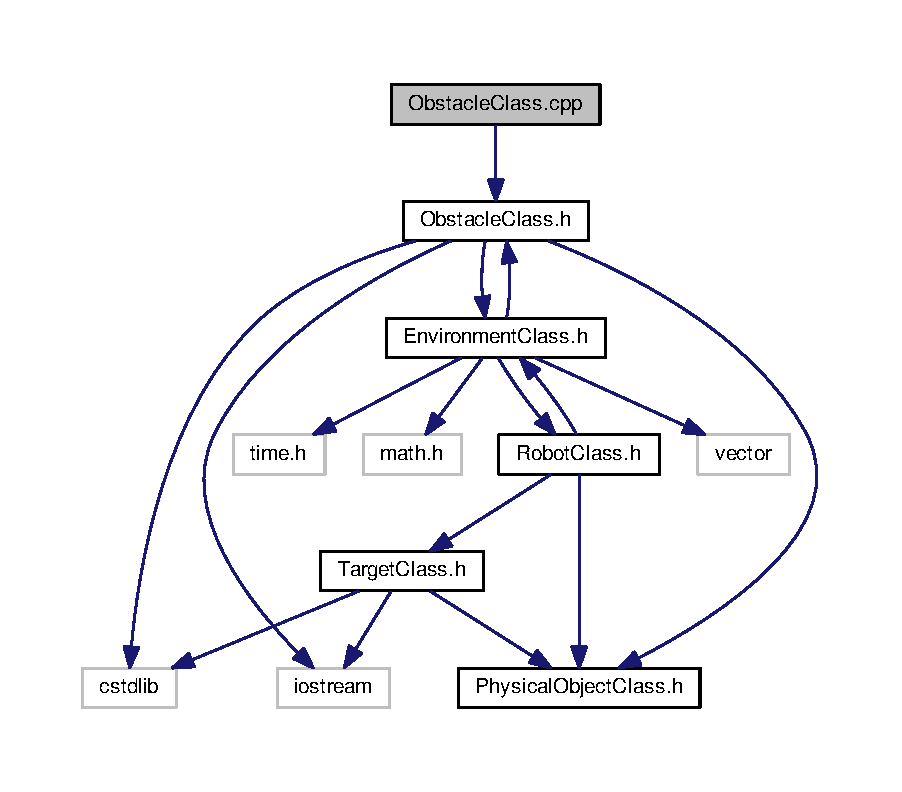
\includegraphics[width=350pt]{ObstacleClass_8cpp__incl}
\end{center}
\end{figure}


\subsection{Detailed Description}
contains \hyperlink{classObstacleClass}{Obstacle\-Class} class definitions \begin{DoxyAuthor}{Author}
Nicholas Inman 

Rachel Soble 

Nicole Zhang 
\end{DoxyAuthor}

\hypertarget{ObstacleClass_8h}{\section{Obstacle\-Class.\-h File Reference}
\label{ObstacleClass_8h}\index{Obstacle\-Class.\-h@{Obstacle\-Class.\-h}}
}


Holds information about obstacles.  


{\ttfamily \#include \char`\"{}Physical\-Object\-Class.\-h\char`\"{}}\\*
{\ttfamily \#include \char`\"{}Environment\-Class.\-h\char`\"{}}\\*
{\ttfamily \#include $<$cstdlib$>$}\\*
{\ttfamily \#include $<$iostream$>$}\\*
Include dependency graph for Obstacle\-Class.\-h\-:
\nopagebreak
\begin{figure}[H]
\begin{center}
\leavevmode
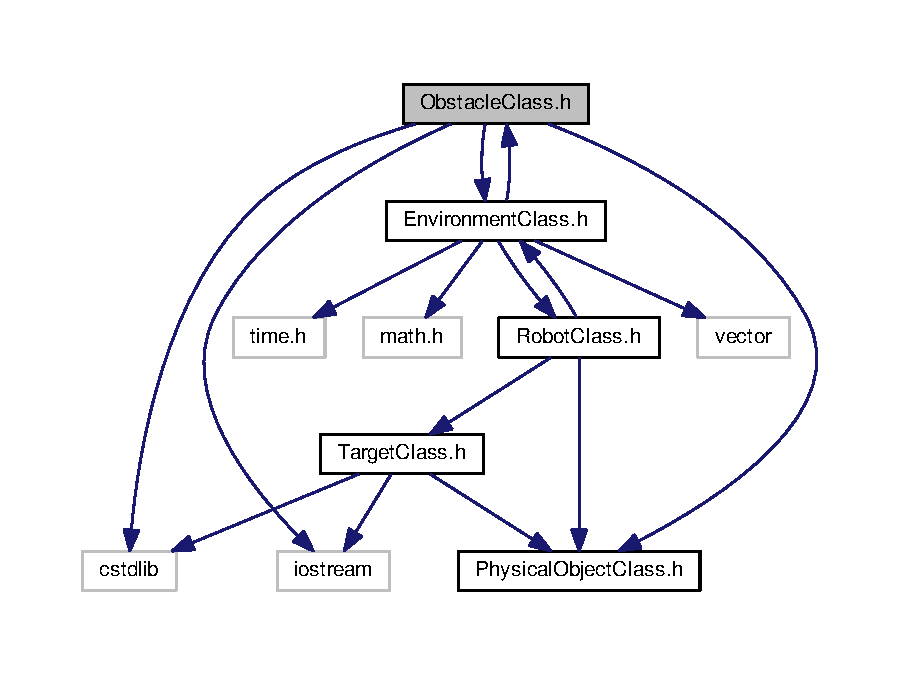
\includegraphics[width=350pt]{ObstacleClass_8h__incl}
\end{center}
\end{figure}
This graph shows which files directly or indirectly include this file\-:
\nopagebreak
\begin{figure}[H]
\begin{center}
\leavevmode
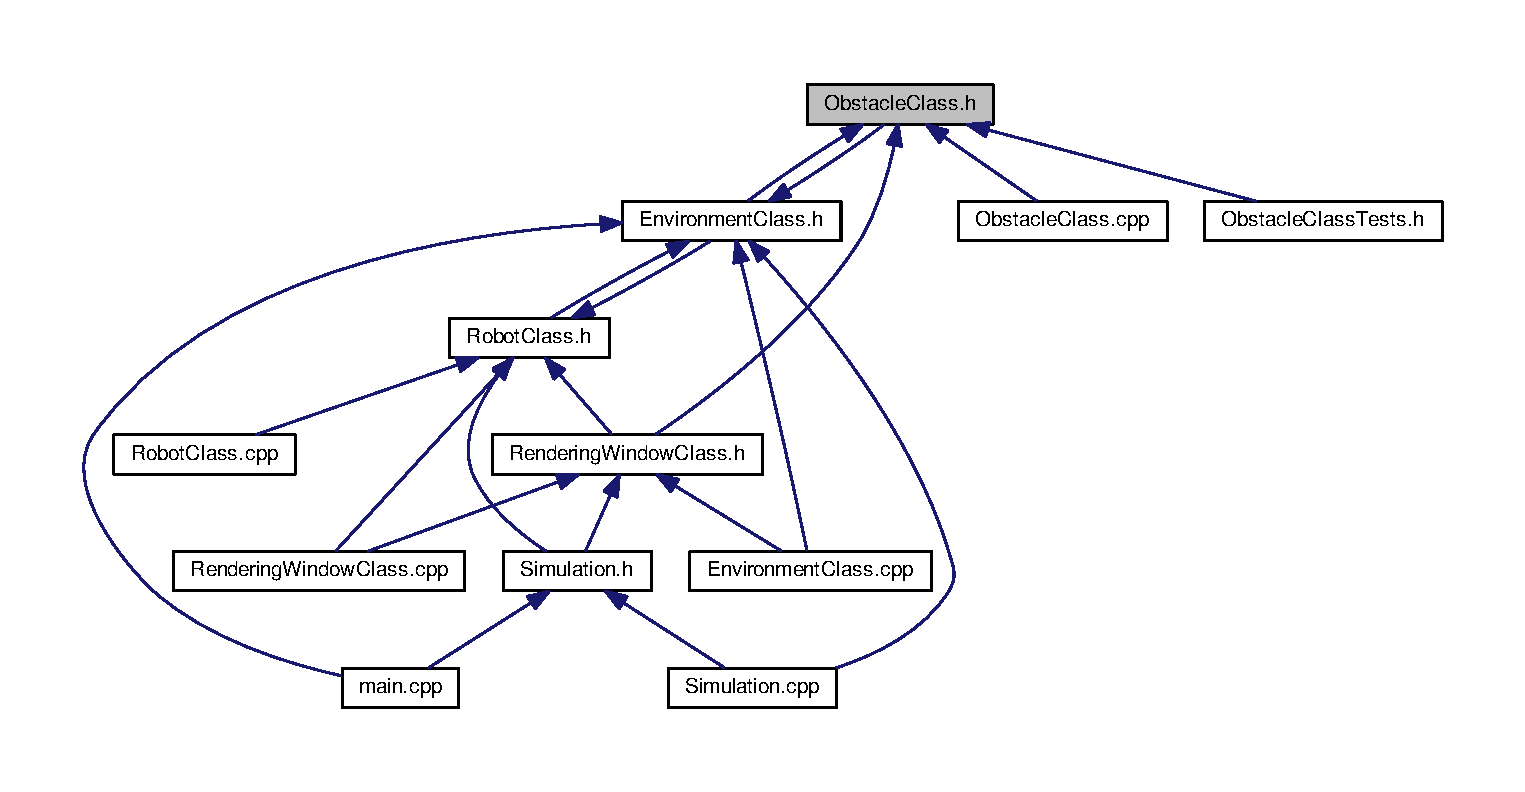
\includegraphics[width=350pt]{ObstacleClass_8h__dep__incl}
\end{center}
\end{figure}
\subsection*{Classes}
\begin{DoxyCompactItemize}
\item 
class \hyperlink{classObstacleClass}{Obstacle\-Class}
\end{DoxyCompactItemize}
\subsection*{Variables}
\begin{DoxyCompactItemize}
\item 
\hypertarget{ObstacleClass_8h_a76b4da66db3ceb6375487da9edcf122b}{\hyperlink{classEnvironmentClass}{Environment\-Class} {\bfseries environment}}\label{ObstacleClass_8h_a76b4da66db3ceb6375487da9edcf122b}

\end{DoxyCompactItemize}


\subsection{Detailed Description}
Holds information about obstacles. 
\hypertarget{PhysicalObjectClass_8cpp}{\section{Physical\-Object\-Class.\-cpp File Reference}
\label{PhysicalObjectClass_8cpp}\index{Physical\-Object\-Class.\-cpp@{Physical\-Object\-Class.\-cpp}}
}


The physical world containing \hyperlink{classRobotClass}{Robot\-Class}, \hyperlink{classTargetClass}{Target\-Class}, and \hyperlink{classObstacleClass}{Obstacle\-Class} objects.  


{\ttfamily \#include \char`\"{}Physical\-Object\-Class.\-h\char`\"{}}\\*
{\ttfamily \#include $<$cstdlib$>$}\\*
{\ttfamily \#include $<$iostream$>$}\\*
Include dependency graph for Physical\-Object\-Class.\-cpp\-:\nopagebreak
\begin{figure}[H]
\begin{center}
\leavevmode
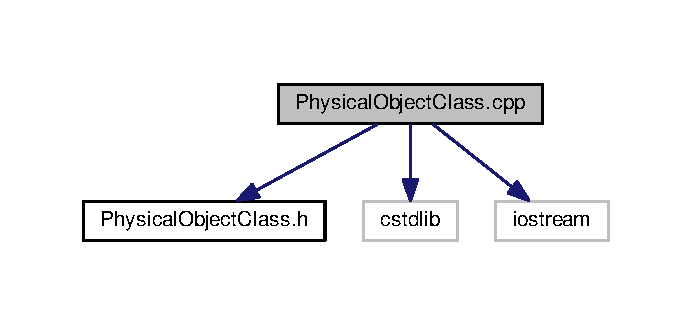
\includegraphics[width=332pt]{PhysicalObjectClass_8cpp__incl}
\end{center}
\end{figure}


\subsection{Detailed Description}
The physical world containing \hyperlink{classRobotClass}{Robot\-Class}, \hyperlink{classTargetClass}{Target\-Class}, and \hyperlink{classObstacleClass}{Obstacle\-Class} objects. \hyperlink{PhysicalObjectClass_8cpp}{Physical\-Object\-Class.\-cpp}

\begin{DoxyAuthor}{Author}
Rachel Soble 
\end{DoxyAuthor}

\hypertarget{PhysicalObjectClass_8h}{\section{Physical\-Object\-Class.\-h File Reference}
\label{PhysicalObjectClass_8h}\index{Physical\-Object\-Class.\-h@{Physical\-Object\-Class.\-h}}
}


The physical world containing \hyperlink{classRobotClass}{Robot\-Class}, \hyperlink{classTargetClass}{Target\-Class}, and \hyperlink{classObstacleClass}{Obstacle\-Class} objects.  


This graph shows which files directly or indirectly include this file\-:
\nopagebreak
\begin{figure}[H]
\begin{center}
\leavevmode
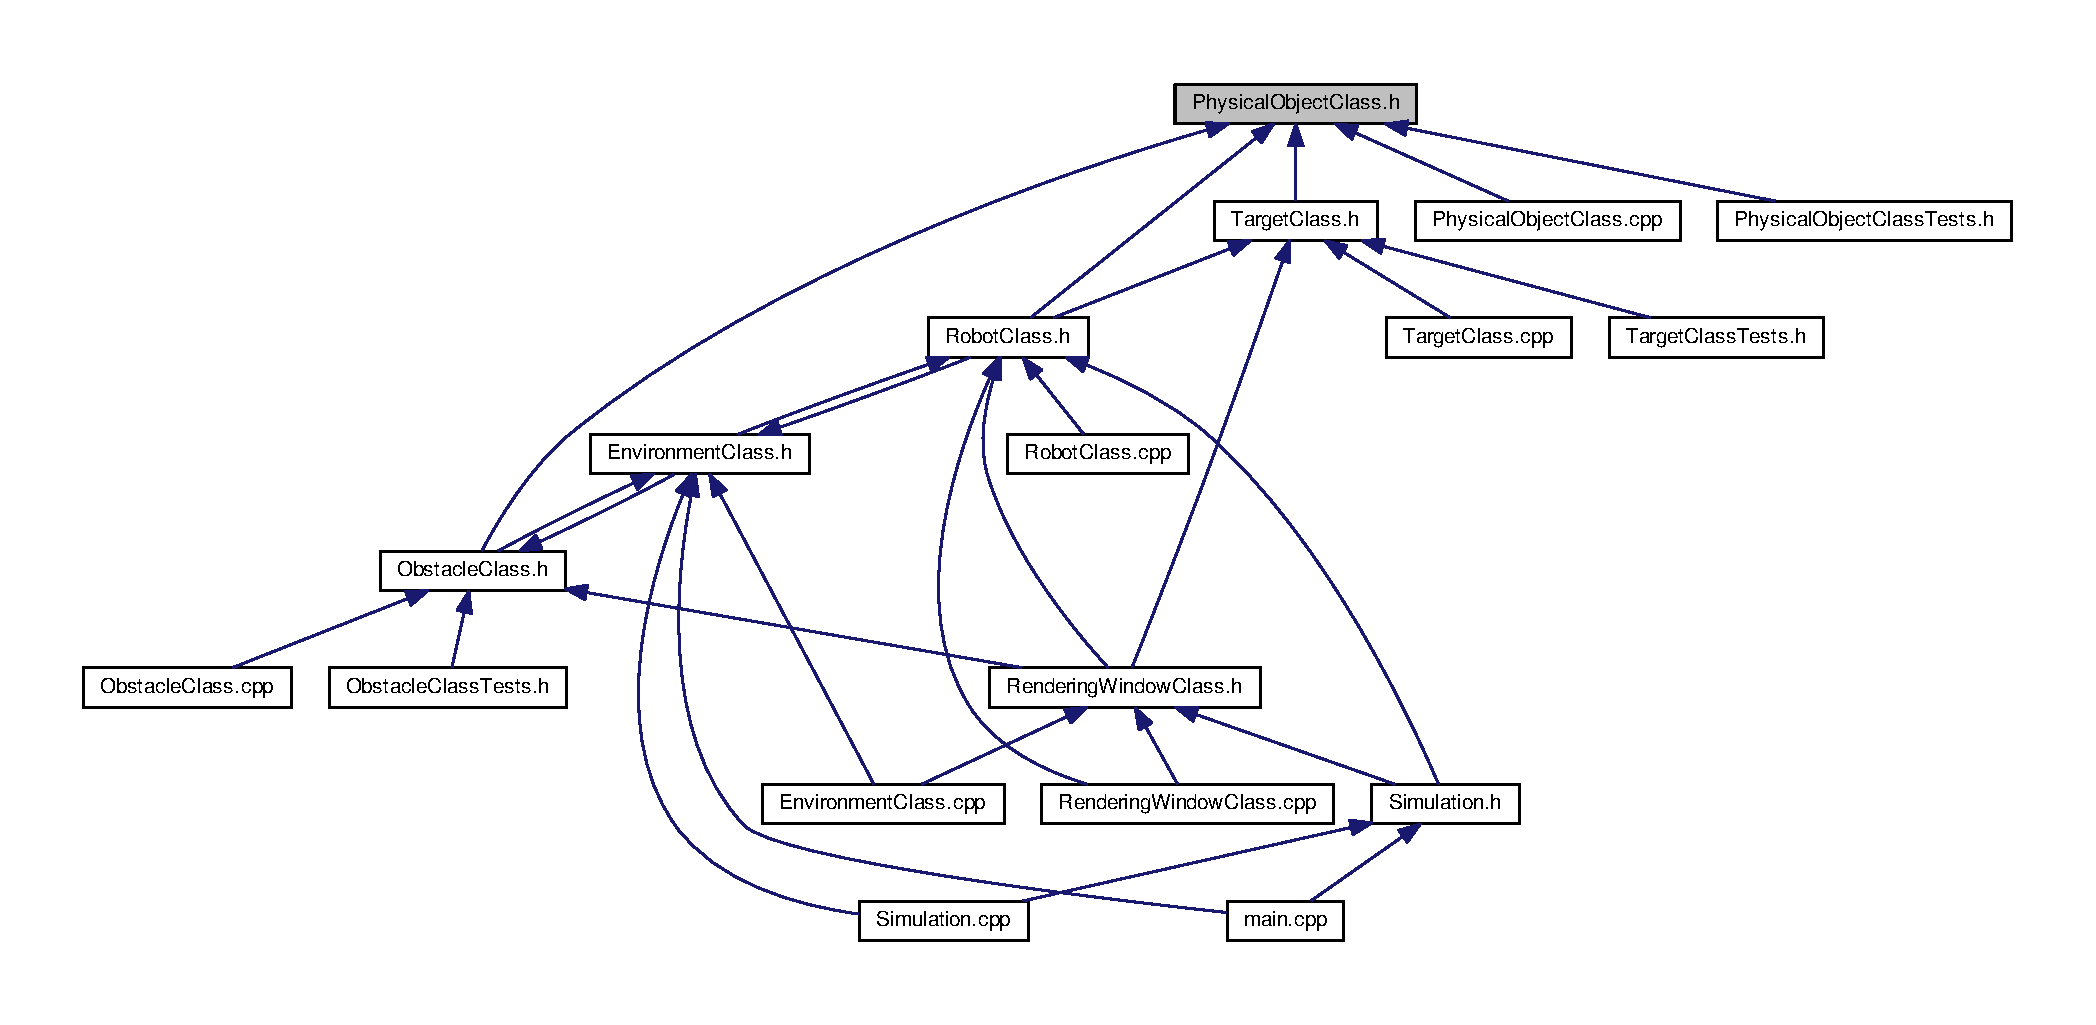
\includegraphics[width=350pt]{PhysicalObjectClass_8h__dep__incl}
\end{center}
\end{figure}
\subsection*{Classes}
\begin{DoxyCompactItemize}
\item 
class \hyperlink{classPhysicalObjectClass}{Physical\-Object\-Class}
\end{DoxyCompactItemize}
\subsection*{Enumerations}
\begin{DoxyCompactItemize}
\item 
enum \hyperlink{PhysicalObjectClass_8h_a842c5e2e69277690b064bf363c017980}{Object\-Type} \{ {\bfseries robot}, 
{\bfseries target}, 
{\bfseries obstacle}
 \}
\begin{DoxyCompactList}\small\item\em Different object types of Physical\-Ojbects. \end{DoxyCompactList}\item 
enum \hyperlink{PhysicalObjectClass_8h_a5a4538eeab397888d88a4eefcc5a1345}{Shape\-Type} \{ {\bfseries square}, 
{\bfseries circle}, 
{\bfseries triangle}
 \}
\begin{DoxyCompactList}\small\item\em Different shape types of Physical\-Ojbects. \end{DoxyCompactList}\end{DoxyCompactItemize}


\subsection{Detailed Description}
The physical world containing \hyperlink{classRobotClass}{Robot\-Class}, \hyperlink{classTargetClass}{Target\-Class}, and \hyperlink{classObstacleClass}{Obstacle\-Class} objects. \hyperlink{PhysicalObjectClass_8h}{Physical\-Object\-Class.\-h}

\begin{DoxyAuthor}{Author}
Rachel Soble 
\end{DoxyAuthor}

\hypertarget{RenderingWindowClass_8cpp}{\section{Rendering\-Window\-Class.\-cpp File Reference}
\label{RenderingWindowClass_8cpp}\index{Rendering\-Window\-Class.\-cpp@{Rendering\-Window\-Class.\-cpp}}
}


Interface between the graphics and \hyperlink{classEnvironmentClass}{Environment\-Class}.  


{\ttfamily \#include \char`\"{}Rendering\-Window\-Class.\-h\char`\"{}}\\*
{\ttfamily \#include \char`\"{}Robot\-Class.\-h\char`\"{}}\\*
{\ttfamily \#include $<$cstdlib$>$}\\*
{\ttfamily \#include $<$iostream$>$}\\*
Include dependency graph for Rendering\-Window\-Class.\-cpp\-:
\nopagebreak
\begin{figure}[H]
\begin{center}
\leavevmode
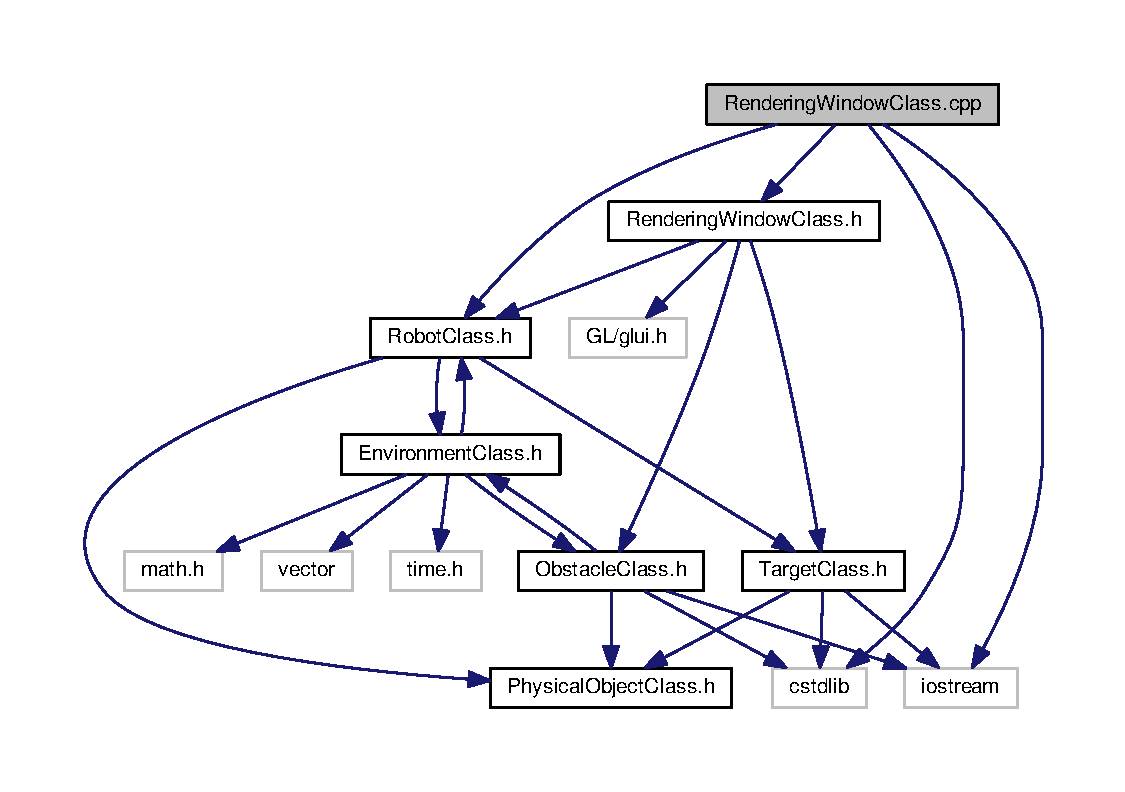
\includegraphics[width=350pt]{RenderingWindowClass_8cpp__incl}
\end{center}
\end{figure}
\subsection*{Macros}
\begin{DoxyCompactItemize}
\item 
\hypertarget{RenderingWindowClass_8cpp_a598a3330b3c21701223ee0ca14316eca}{\#define {\bfseries P\-I}~3.\-14f}\label{RenderingWindowClass_8cpp_a598a3330b3c21701223ee0ca14316eca}

\end{DoxyCompactItemize}


\subsection{Detailed Description}
Interface between the graphics and \hyperlink{classEnvironmentClass}{Environment\-Class}. \hyperlink{RenderingWindowClass_8cpp}{Rendering\-Window\-Class.\-cpp} 
\hypertarget{RenderingWindowClass_8h}{\section{Rendering\-Window\-Class.\-h File Reference}
\label{RenderingWindowClass_8h}\index{Rendering\-Window\-Class.\-h@{Rendering\-Window\-Class.\-h}}
}


Interface between the graphics and \hyperlink{classEnvironmentClass}{Environment\-Class}.  


{\ttfamily \#include $<$G\-L/glui.\-h$>$}\\*
{\ttfamily \#include \char`\"{}Robot\-Class.\-h\char`\"{}}\\*
{\ttfamily \#include \char`\"{}Target\-Class.\-h\char`\"{}}\\*
{\ttfamily \#include \char`\"{}Obstacle\-Class.\-h\char`\"{}}\\*
Include dependency graph for Rendering\-Window\-Class.\-h\-:
\nopagebreak
\begin{figure}[H]
\begin{center}
\leavevmode
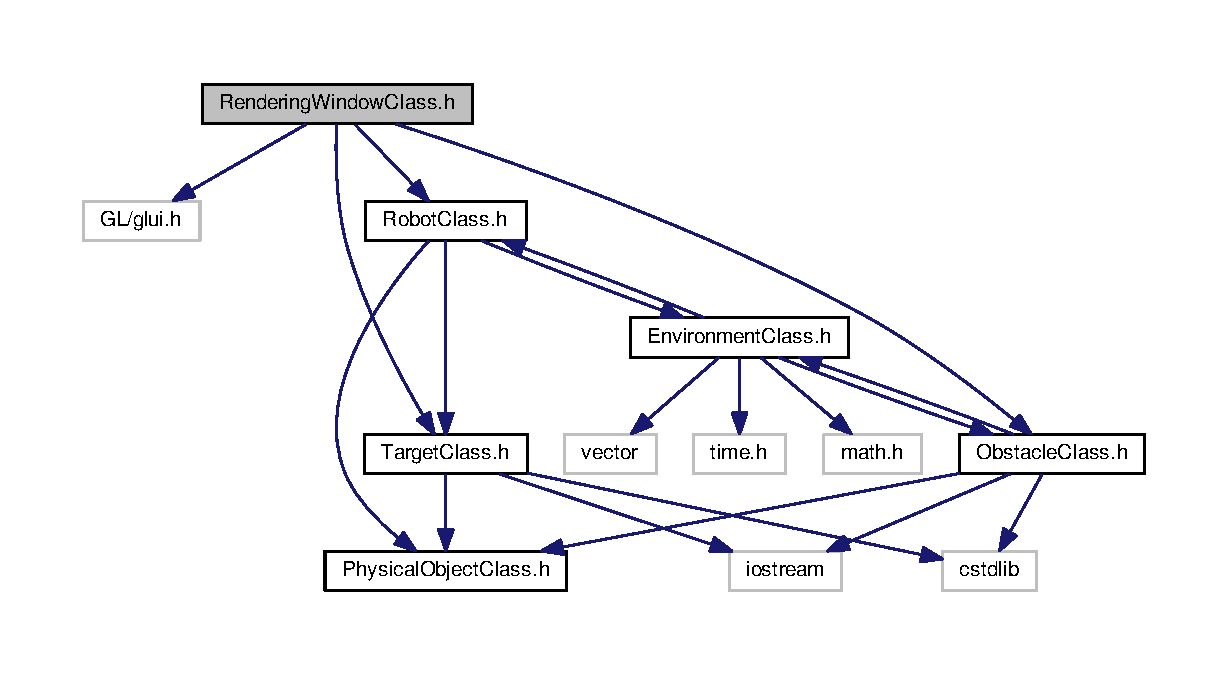
\includegraphics[width=350pt]{RenderingWindowClass_8h__incl}
\end{center}
\end{figure}
This graph shows which files directly or indirectly include this file\-:
\nopagebreak
\begin{figure}[H]
\begin{center}
\leavevmode
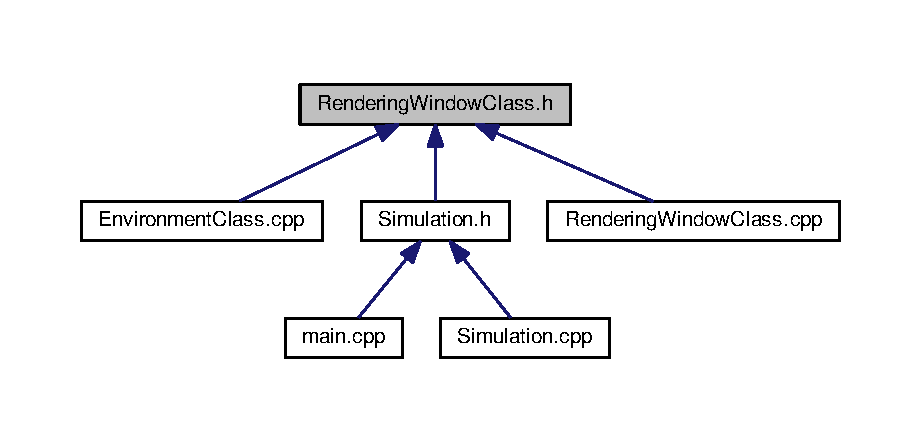
\includegraphics[width=350pt]{RenderingWindowClass_8h__dep__incl}
\end{center}
\end{figure}
\subsection*{Classes}
\begin{DoxyCompactItemize}
\item 
class \hyperlink{classRenderingWindowClass}{Rendering\-Window\-Class}
\end{DoxyCompactItemize}


\subsection{Detailed Description}
Interface between the graphics and \hyperlink{classEnvironmentClass}{Environment\-Class}. \hyperlink{RenderingWindowClass_8h}{Rendering\-Window\-Class.\-h} 
\hypertarget{RobotClass_8cpp}{\section{Robot\-Class.\-cpp File Reference}
\label{RobotClass_8cpp}\index{Robot\-Class.\-cpp@{Robot\-Class.\-cpp}}
}


contains Drawing class definitions  


{\ttfamily \#include \char`\"{}Robot\-Class.\-h\char`\"{}}\\*
Include dependency graph for Robot\-Class.\-cpp\-:
\nopagebreak
\begin{figure}[H]
\begin{center}
\leavevmode
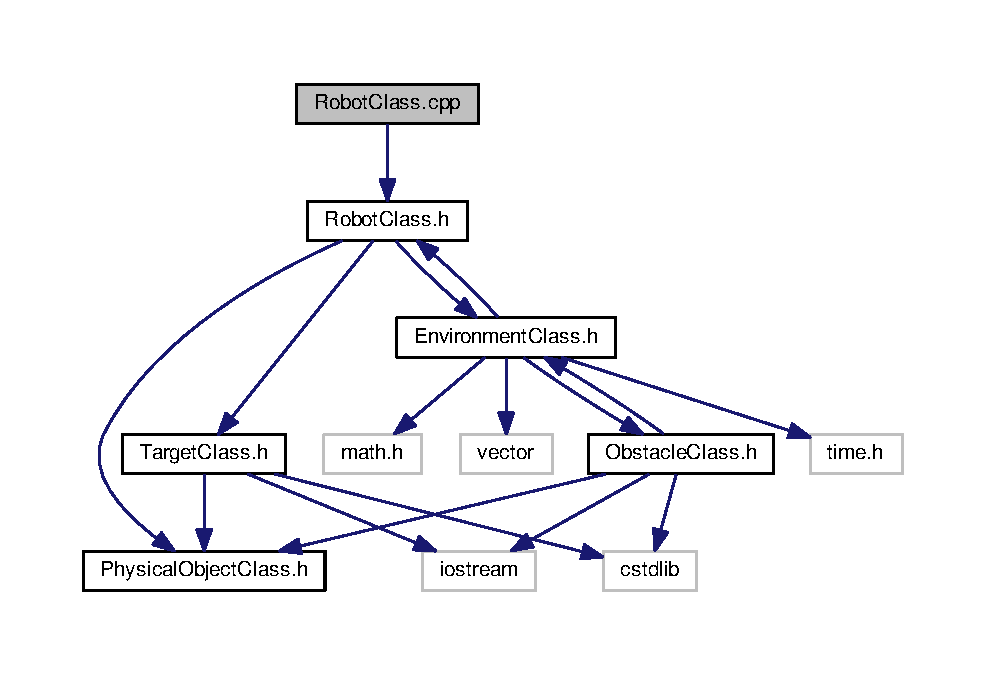
\includegraphics[width=350pt]{RobotClass_8cpp__incl}
\end{center}
\end{figure}


\subsection{Detailed Description}
contains Drawing class definitions \hyperlink{RobotClass_8cpp}{Robot\-Class.\-cpp} \begin{DoxyAuthor}{Author}
Rachel Soble 

Nicholas Inman 
\end{DoxyAuthor}

\hypertarget{RobotClass_8h}{\section{Robot\-Class.\-h File Reference}
\label{RobotClass_8h}\index{Robot\-Class.\-h@{Robot\-Class.\-h}}
}


The representation of the robot within the simulation.  


{\ttfamily \#include \char`\"{}Physical\-Object\-Class.\-h\char`\"{}}\\*
{\ttfamily \#include \char`\"{}Target\-Class.\-h\char`\"{}}\\*
{\ttfamily \#include \char`\"{}Environment\-Class.\-h\char`\"{}}\\*
Include dependency graph for Robot\-Class.\-h\-:
\nopagebreak
\begin{figure}[H]
\begin{center}
\leavevmode
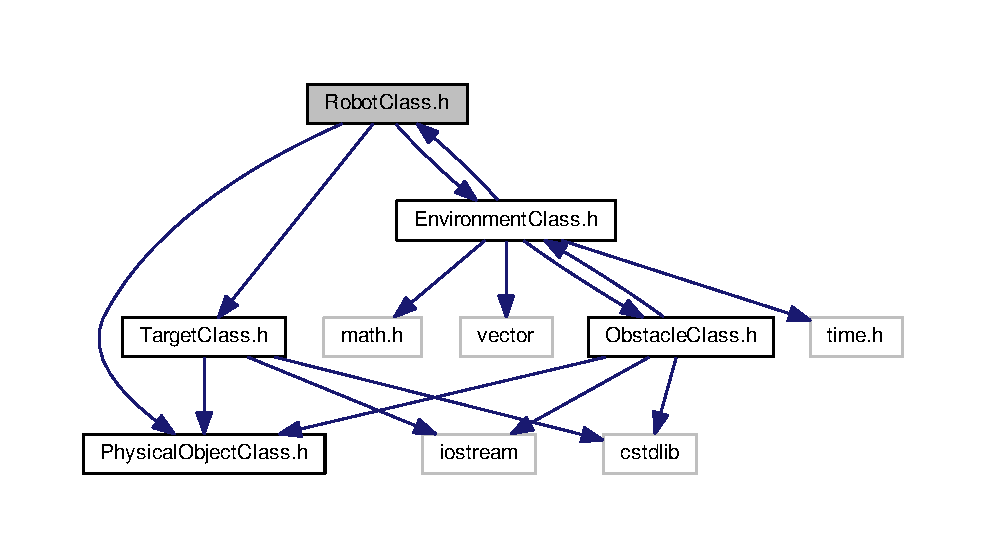
\includegraphics[width=350pt]{RobotClass_8h__incl}
\end{center}
\end{figure}
This graph shows which files directly or indirectly include this file\-:
\nopagebreak
\begin{figure}[H]
\begin{center}
\leavevmode
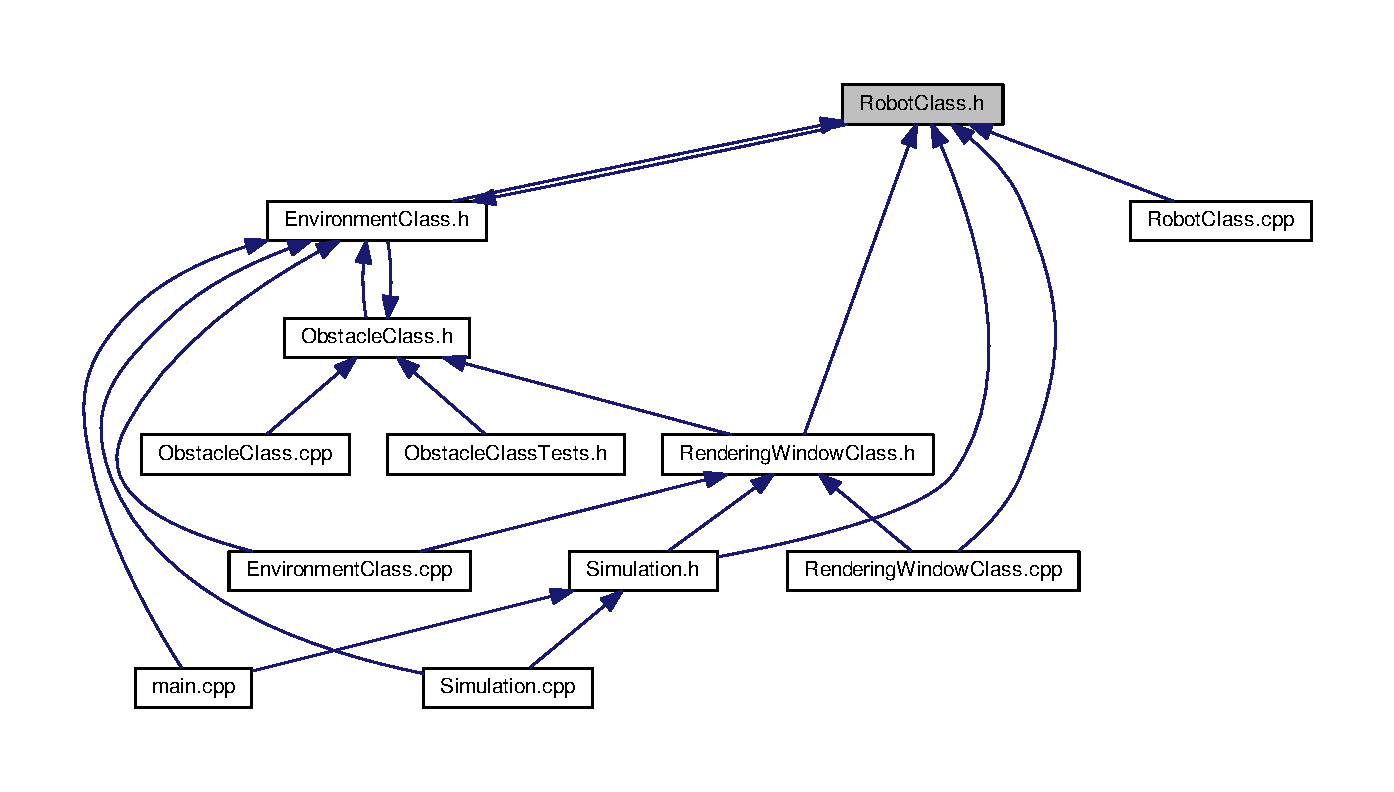
\includegraphics[width=350pt]{RobotClass_8h__dep__incl}
\end{center}
\end{figure}
\subsection*{Classes}
\begin{DoxyCompactItemize}
\item 
class \hyperlink{classRobotClass}{Robot\-Class}
\end{DoxyCompactItemize}
\subsection*{Variables}
\begin{DoxyCompactItemize}
\item 
\hypertarget{RobotClass_8h_a76b4da66db3ceb6375487da9edcf122b}{\hyperlink{classEnvironmentClass}{Environment\-Class} {\bfseries environment}}\label{RobotClass_8h_a76b4da66db3ceb6375487da9edcf122b}

\end{DoxyCompactItemize}


\subsection{Detailed Description}
The representation of the robot within the simulation. \hyperlink{RobotClass_8h}{Robot\-Class.\-h} \begin{DoxyAuthor}{Author}
Rachel Soble, soble004, Group 5
\end{DoxyAuthor}
Adapted from class sample 
\hypertarget{Simulation_8cpp}{\section{Simulation.\-cpp File Reference}
\label{Simulation_8cpp}\index{Simulation.\-cpp@{Simulation.\-cpp}}
}


contains \hyperlink{classSimulation}{Simulation} class definitions  


{\ttfamily \#include \char`\"{}Simulation.\-h\char`\"{}}\\*
{\ttfamily \#include \char`\"{}Environment\-Class.\-h\char`\"{}}\\*
Include dependency graph for Simulation.\-cpp\-:
\nopagebreak
\begin{figure}[H]
\begin{center}
\leavevmode
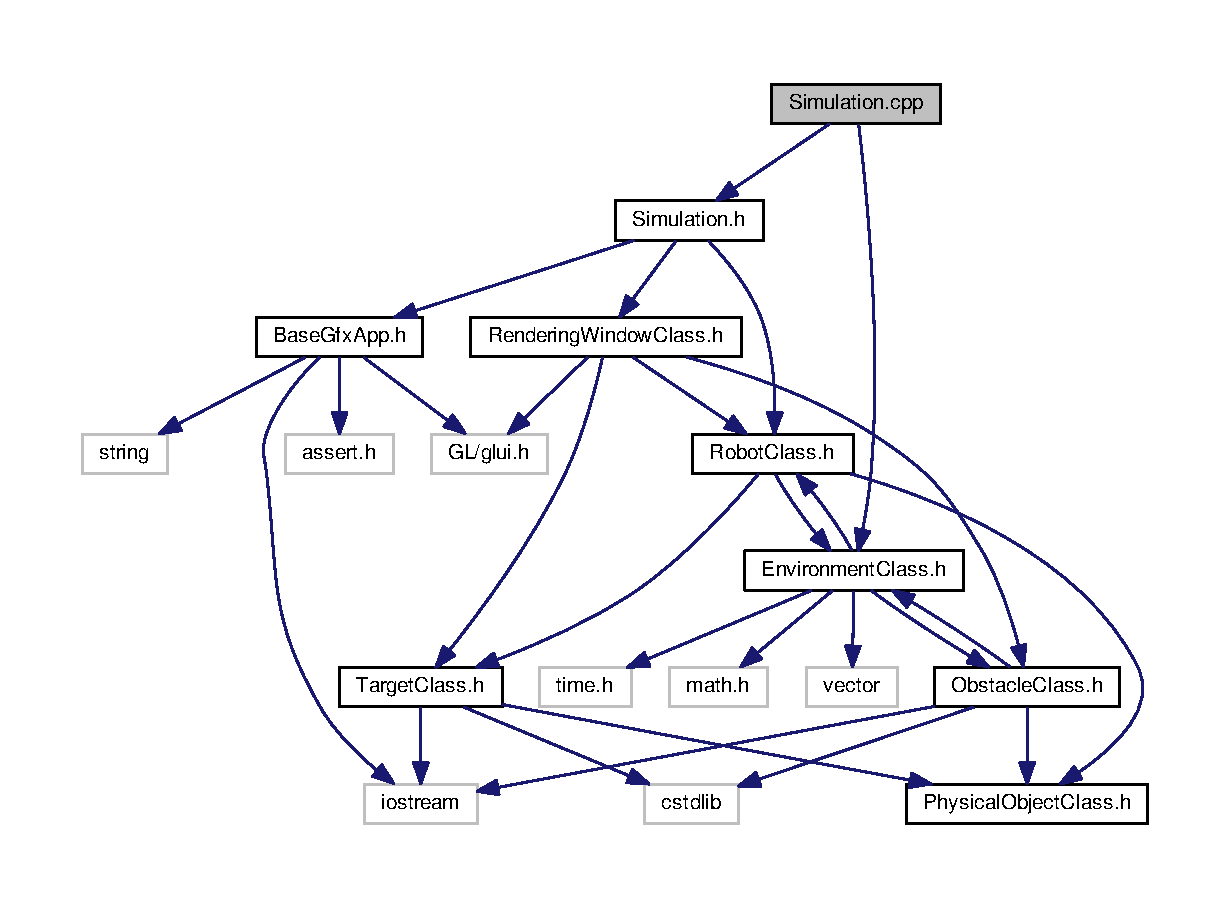
\includegraphics[width=350pt]{Simulation_8cpp__incl}
\end{center}
\end{figure}
\subsection*{Macros}
\begin{DoxyCompactItemize}
\item 
\hypertarget{Simulation_8cpp_a598a3330b3c21701223ee0ca14316eca}{\#define {\bfseries P\-I}~3.\-14}\label{Simulation_8cpp_a598a3330b3c21701223ee0ca14316eca}

\end{DoxyCompactItemize}
\subsection*{Variables}
\begin{DoxyCompactItemize}
\item 
\hypertarget{Simulation_8cpp_adf916204820072417ed73a32de1cefcf}{int {\bfseries flag}}\label{Simulation_8cpp_adf916204820072417ed73a32de1cefcf}

\item 
\hypertarget{Simulation_8cpp_a096533d53bd51a3ea732f287f8dbf003}{double {\bfseries past\-Time}}\label{Simulation_8cpp_a096533d53bd51a3ea732f287f8dbf003}

\end{DoxyCompactItemize}


\subsection{Detailed Description}
contains \hyperlink{classSimulation}{Simulation} class definitions \begin{DoxyAuthor}{Author}
Nicole Zhang 

Rachel Soble 

Nicholas Inman 
\end{DoxyAuthor}

\hypertarget{Simulation_8h}{\section{Simulation.\-h File Reference}
\label{Simulation_8h}\index{Simulation.\-h@{Simulation.\-h}}
}


Main application class for the robot simulation.  


{\ttfamily \#include \char`\"{}Base\-Gfx\-App.\-h\char`\"{}}\\*
{\ttfamily \#include \char`\"{}Robot\-Class.\-h\char`\"{}}\\*
{\ttfamily \#include \char`\"{}Rendering\-Window\-Class.\-h\char`\"{}}\\*
Include dependency graph for Simulation.\-h\-:
\nopagebreak
\begin{figure}[H]
\begin{center}
\leavevmode
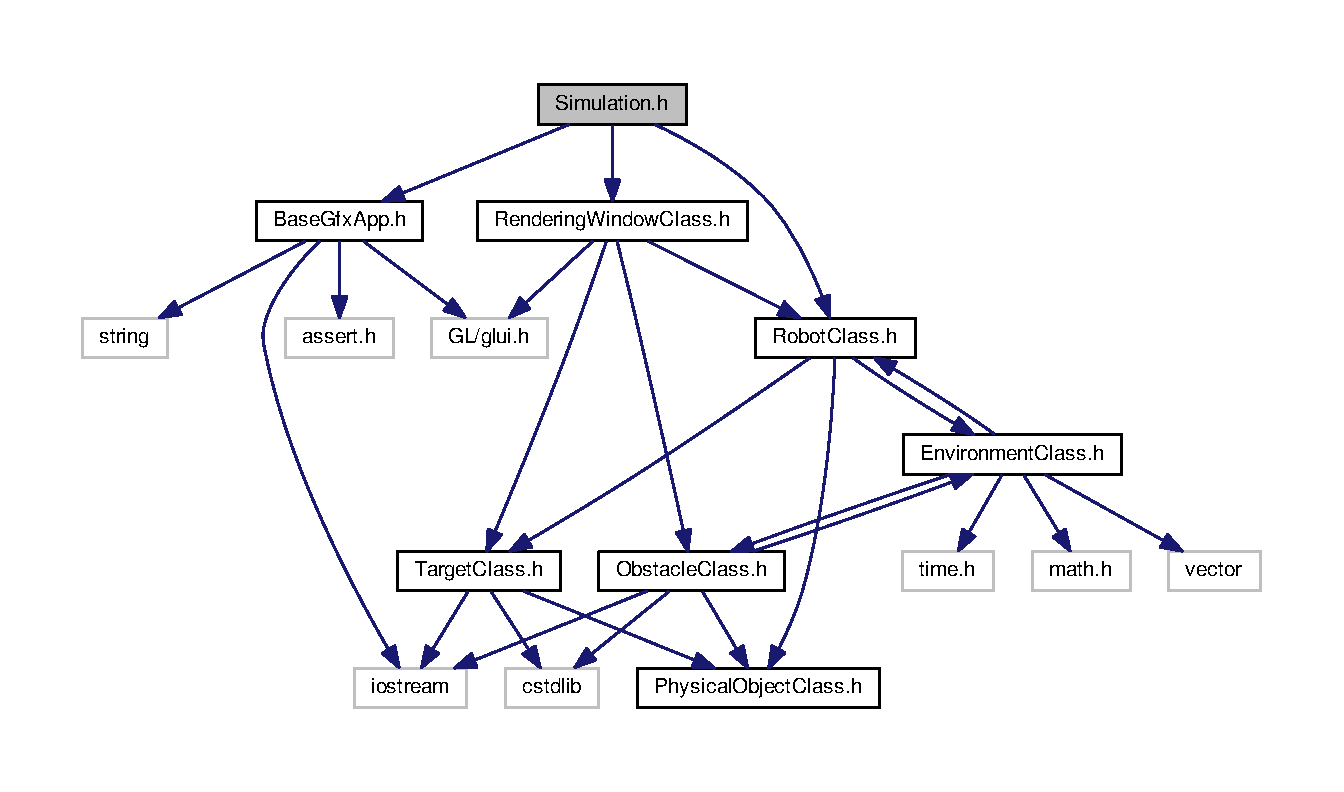
\includegraphics[width=350pt]{Simulation_8h__incl}
\end{center}
\end{figure}
This graph shows which files directly or indirectly include this file\-:\nopagebreak
\begin{figure}[H]
\begin{center}
\leavevmode
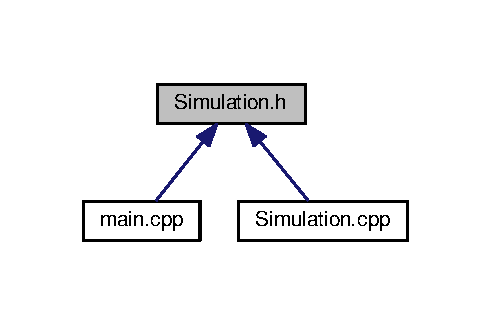
\includegraphics[width=235pt]{Simulation_8h__dep__incl}
\end{center}
\end{figure}
\subsection*{Classes}
\begin{DoxyCompactItemize}
\item 
class \hyperlink{classSimulation}{Simulation}
\end{DoxyCompactItemize}
\subsection*{Variables}
\begin{DoxyCompactItemize}
\item 
\hypertarget{Simulation_8h_a76b4da66db3ceb6375487da9edcf122b}{\hyperlink{classEnvironmentClass}{Environment\-Class} {\bfseries environment}}\label{Simulation_8h_a76b4da66db3ceb6375487da9edcf122b}

\end{DoxyCompactItemize}


\subsection{Detailed Description}
Main application class for the robot simulation. \begin{DoxyAuthor}{Author}
Nicole Zhang 

Nicholas Inman 
\end{DoxyAuthor}

\hypertarget{TargetClass_8cpp}{\section{Target\-Class.\-cpp File Reference}
\label{TargetClass_8cpp}\index{Target\-Class.\-cpp@{Target\-Class.\-cpp}}
}


contains Target class definitions  


{\ttfamily \#include \char`\"{}Target\-Class.\-h\char`\"{}}\\*
Include dependency graph for Target\-Class.\-cpp\-:\nopagebreak
\begin{figure}[H]
\begin{center}
\leavevmode
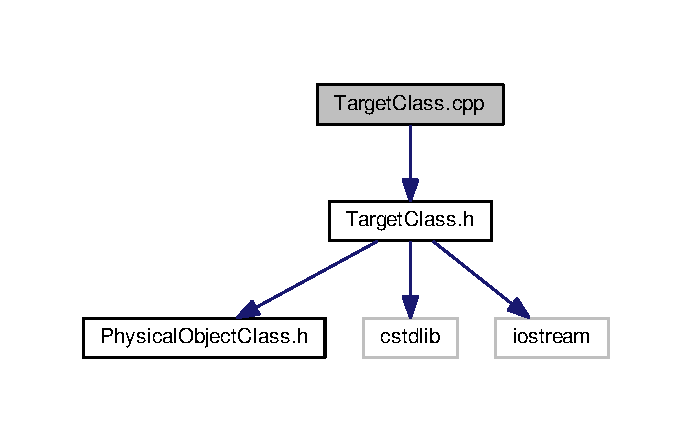
\includegraphics[width=332pt]{TargetClass_8cpp__incl}
\end{center}
\end{figure}


\subsection{Detailed Description}
contains Target class definitions 
\hypertarget{TargetClass_8h}{\section{Target\-Class.\-h File Reference}
\label{TargetClass_8h}\index{Target\-Class.\-h@{Target\-Class.\-h}}
}


Holds information about targets.  


{\ttfamily \#include \char`\"{}Physical\-Object\-Class.\-h\char`\"{}}\\*
{\ttfamily \#include $<$cstdlib$>$}\\*
{\ttfamily \#include $<$iostream$>$}\\*
Include dependency graph for Target\-Class.\-h\-:\nopagebreak
\begin{figure}[H]
\begin{center}
\leavevmode
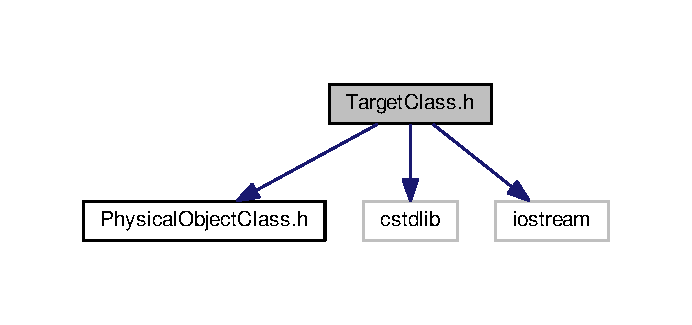
\includegraphics[width=332pt]{TargetClass_8h__incl}
\end{center}
\end{figure}
This graph shows which files directly or indirectly include this file\-:
\nopagebreak
\begin{figure}[H]
\begin{center}
\leavevmode
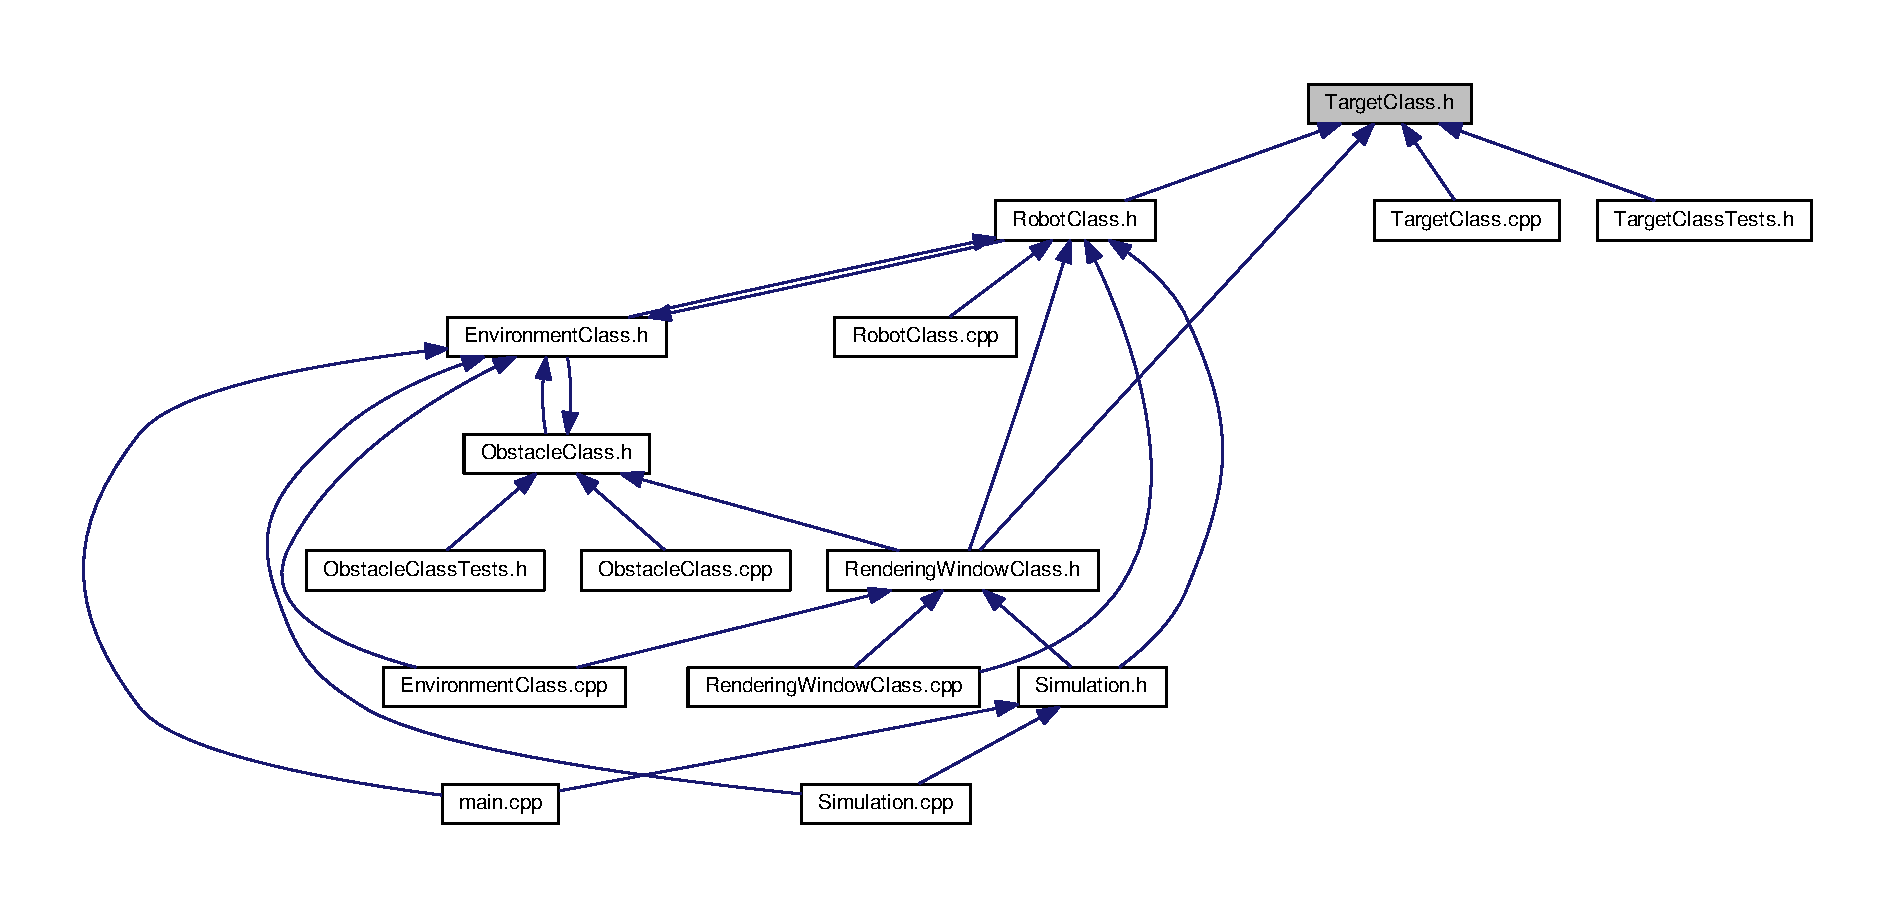
\includegraphics[width=350pt]{TargetClass_8h__dep__incl}
\end{center}
\end{figure}
\subsection*{Classes}
\begin{DoxyCompactItemize}
\item 
class \hyperlink{classTargetClass}{Target\-Class}
\end{DoxyCompactItemize}


\subsection{Detailed Description}
Holds information about targets. 
%--- End generated contents ---

% Index
\newpage
\phantomsection
\addcontentsline{toc}{chapter}{Index}
\printindex

\end{document}
